%%%%%%%%%%%%%%%%%%%%%%%%%%%%%%%%%%%%%%
%% Header section of Latex document %%
%%%%%%%%%%%%%%%%%%%%%%%%%%%%%%%%%%%%%%

\documentclass[a4paper]{report}
%% @author Daniel Lukacs, dlukacs@caesar.elte.hu, 2017

\usepackage[a4paper]{geometry}
\usepackage{t1enc}
\usepackage[utf8]{inputenc}
\usepackage{lmodern}

\usepackage[title,titletoc]{appendix}
\usepackage[section]{placeins}
\usepackage{relsize}

\usepackage[normalem]{ulem} %% Provides underlining.
\usepackage{caption} %% Provides captions.
\usepackage{mdframed} %% Provides frames around text and equations.
\usepackage{tikz-cd} %% Provides diagram drawing environment.
\usepackage{adjustbox} %% Provides additional tools to resize content.
% \usepackage[magyar]{babel} %% Provides foreign language support.

%%%%
%% Provides math related environments and directives.
\usepackage{amssymb}
\usepackage{amsthm}
\usepackage{amsmath}
\usepackage{latexsym}

%% See http://tex.stackexchange.com/questions/43835/conflict-between-amsthm-and-some-other-package
\let\proof\relax 
\let\endproof\relax

%%%%
%% Provides table environments and related directives.
\usepackage{array}
\usepackage{tabulary}
\usepackage{tabularx}
\usepackage{multirow}
\usepackage{hhline}

%%%%
%% Provides figure environments and related directives.
\usepackage{graphicx}
\makeatletter
\def\maxwidth#1{\ifdim\Gin@nat@width>#1 #1\else\Gin@nat@width\fi}
\def\maxheight#1{\ifdim\Gin@nat@height>#1 #1\else\Gin@nat@height\fi}
\makeatother

%%\usepackage{fancyvrb}
\usepackage{rotating}

%%%%
%% Provides environment to display source code.
\usepackage{listings} 
\lstset{ 
    literate=%
        {á}{{\'a}}1
        {é}{{\'e}}1
        {í}{{\'i}}1
        {ó}{{\'o}}1
        {ö}{{\"o}}1
        {ő}{{\H{o}}}1
        {ú}{{\'u}}1
        {ü}{{\"u}}1
        {ű}{{\H{u}}}1
        {Á}{{\'A}}1
        {É}{{\'E}}1
        {Í}{{\'I}}1
        {Ó}{{\'O}}1
        {Ö}{{\"O}}1
        {Ő}{{\H{O}}}1
        {Ú}{{\'U}}1
        {Ü}{{\"U}}1
        {Ű}{{\H{U}}}1
    } %% Customization of listings env., to enable non-English accents.

\lstset{
   frame=single,
   basicstyle=\small,
   language=Erlang,
   numbers=left,
   firstnumber=1,
   numberfirstline=true,
%  basicstyle=\ttfamily,
%  columns=fullflexible,
%   keepspaces=true,
} %% Customization of listings environment


%%%%
%% Provides environment to display pseudocode.
\usepackage{algorithm}% http://ctan.org/pkg/algorithms
\usepackage{algpseudocode}% http://ctan.org/pkg/algorithmicx

\newcommand{\repeatcaption}[2]{%
  \addtocounter{figure}{-1}%
  \renewcommand{\thefigure}{\ref{#1}}%
  \captionsetup{list=no, labelformat=simple, labelsep=colon}%
  \captionof{figure}{#2}%
} %% Customization: Using the same figure twice with no new number. See http://tex.stackexchange.com/a/200229

%%%%
%% Provides directives to display followable URL references.
\usepackage{url}
\usepackage{hyperref}
\hypersetup{
  hidelinks,
  linkbordercolor = {0 0 1},
}

%% Customization: Followable links to appendix references.
\makeatletter
\appto{\appendices}{\def\Hy@chapapp{Appendix}}
\makeatother


%%%%
%% Custom document formatting.

% \renewcommand{\abstract}{ \begin{center}\textbf{Abstract}\end{center}}

\setcounter{tocdepth}{2}

\setlength{\parskip}{\baselineskip}%
\setlength{\parindent}{0pt}%

\makeatletter
\renewcommand\subsubsection{\@startsection{subsubsection}{3}{\z@}%
                       {-18\p@ \@plus -4\p@ \@minus -4\p@}%
                       {4\p@ \@plus 2\p@ \@minus 2\p@}%
                       {\normalfont\normalsize\bfseries\boldmath
                        \rightskip=\z@ \@plus 8em\pretolerance=10000 }}
\makeatother


%%%%
%% Custom theorem environments.
\newtheorem{mydef}{Definition}
\newtheorem{myexamp}{Example}

%%%%
%% Custom symbol definitions and abbreviations.
\makeatletter
\providecommand{\leadsfrom}{%
  \mathrel{\mathpalette\reflect@squig\relax}%
}
\newcommand{\reflect@squig}[2]{%
  \reflectbox{$\m@th#1\leadsto$}%
}
\makeatother

\renewcommand{\labelitemi}{$\circ$}
\newcommand{\edge}[1]{\stackrel{\bf{#1}}{\rightarrow}}
\newcommand{\ledge}[1]{\stackrel{\bf{#1}}{\leftarrow}}
\newcommand{\rel}[1]{\stackrel{\bf{#1}}{\leadsto}}
\newcommand{\trel}[1]{\stackrel{\bf{#1}}{\leadsto^*}}
\newcommand{\lrel}[1]{\stackrel{\bf{#1}}{\leadsfrom}}

\newcommand{\eqname}[1]{\tag*{#1}}% Tag equation with name

\newcommand{\nv}[0]{node(v)}
\newcommand{\ruleref}[1]{(\S\ref{#1})}
\newcommand{\apxref}[1]{(Appendix \ref{#1}.)}
\newcommand{\apxrefm}[3]{(Appendix \ref{#1}., \ref{#2}. és \ref{#3}.)}
\renewcommand{\_}{\textunderscore\hspace{0pt}}


\hyphenation{Re-fac-tor-Erl}

%%%%%%%%%%%%%%%%%%%%%%%%%%%%%%%%%%%%
%% Body section of Latex document %%
%%%%%%%%%%%%%%%%%%%%%%%%%%%%%%%%%%%%

\begin{document}
% \title{The title of your thesis}
% \thispagestyle{empty}
% \begin{center}
% {\Huge TDK dolgozat}\\[0.5cm]
% {\bf Név} \\[1cm]
% \end{center}


\begin{titlepage}
  \noindent
  \begin{minipage}{0.25 \textwidth}
    
\includegraphics[height=40mm]{figures/cimer.png}
  \end{minipage}
  \hfill
  \begin{minipage}{0.67 \textwidth}
    \large
    Eötvös Loránd University \\
    Faculty of Informatics \\
    Department of Programming Languages and Compilers \\
    
  \end{minipage}

  \vfill

  \begin{center}
    {\LARGE \bfseries Analysing the changes of software metric values with RefactorErl}
    %% \\[1.5cm]
    %% {\Large TDK dolgozat}
    %% \\[3cm]
    \\[6cm]
    \begin{minipage}[t]{0.45 \textwidth}
      \emph{Supervisor:} \\[0.25 \baselineskip]
      {\large Melinda Tóth} \\[0.5 \baselineskip]
      Assistant lecturer
    \end{minipage}
    \begin{minipage}[t]{0.45 \textwidth}
      \begin{flushright}
        \emph{Author:} \\[0.25 \baselineskip]
        {\large Marina Konoreva} \\[0.5 \baselineskip]
        Computer Science MSc \\ %% The name of your program
        2. year
      \end{flushright}
    \end{minipage}
  \end{center}

  \vfill

  \begin{center}
    \large Budapest, 2019
  \end{center}
\end{titlepage}

%%%%%%%%%%%%%%%%%%%%%%%%%%%%%%%%%
%% Content sections start here %%

\begin{abstract}
%% While you can write all your content here in the main file, it's recommended
%%   to keep your content into separate files. The \input directive simply
%%   copies here the text of the pointed line.
This page contains the text of your abstract.


\end{abstract}

\tableofcontents

\chapter{Introduction}
Requirements for the quality of the product being developed have rapidly increased in recent years. From the beginning of software product development, developers have been striving to monitor quality. Software metrics and their visualization are two important features of measurement systems. 

In this thesis, we introduce framework for analysing of quality of programs written in the Erlang programing language which built on the top of the RefactorErl static analyzis tool. Our goal is to analyse
projects and then prepare the results of the measurements.

Erlang is a functional language designed for highly parallel, scalable applications requiring high uptime. Several industrial and open source products were implemented in Erlang, therefor tools to measure the complexity, qulity of the source code are highly desirable. 

RefactorErl is a static source code analysis and transformation tool for Erlang providing several software metrics. The tool is developed by the Department of Programming Languages and Compilers at the Faculty of Informatics, Eötvös Loránd University, Budapest, Hungary. 
Among the features of RefactorErl is included a metric query language which can support Erlang developers in everyday tasks such as program comprehension, debugging, finding relationships among program parts, etc.
Software metrics provide a means to extract useful and measurable information about the structure of a software system.
The results of these evaluation methods can be used to indicate which parts of a software system need to be reengineered.

This thesis is organized as follows: Chapter 2 is needed for understand-
ing the main concepts of software metrics. Chapter 3 covers the necessary background on Erlang programming language, RefactorErl tool, defined metrics  in this tool and description developed framework. Chapter 4 illustrates measurements and findings of some projects. Chapter 5 describes some related works. Chapter 6 consists conclusion about complited work.



\chapter{Software metrics}
This chapter presents the introduction to the software metrics as the key point for evaluation of productivity and quality of the software development product. There is also classification of the software metrics, description the different measurements of software metrics in general and the most popular software metrics tools.


\section{Definition of Software Metrics}

Software metrics are the attributes of the software systems that deals with the measurements of the software product and process by which it is developed~\cite{metrix}.
 
A software metric is a measure of software characteristics which are quantifiable or countable. Software metrics are important for many reasons, including measuring software performance, planning work items, measuring productivity, and many other uses.

Software developers must recognize the principles of software metrics that involve cost,schedule find quality goals, quantitative goals, comparison of plans with actual performance throughout development, monitoring data trends for indication of likely problems, metrics presentation, and investigation of data values.

Within the software development process, there are many metrics that are all related to each other. Metrics are related to the four functions of management:

\begin{itemize}
	\item Planning.
	\item Organising.
	\item Controlling.
	\item Improving.
\end{itemize}

The goal of tracking and analyzing software metrics is to determine the quality of the current product or process, improve that quality and predict the quality once the software development project is complete. On a more granular level, software development managers are trying to:

\begin{itemize}
	\item Increase return on investment (ROI).
	\item Identify areas of improvement.
	\item Manage workloads.
	\item Reduce overtime.
	\item Reduce costs.
\end{itemize}

These goals can be achieved by providing information and clarity throughout the organization about complex software development projects. Metrics are an important component of quality assurance, management, debugging, performance, and estimating costs,and they’re valuable for both developers and development team leaders:

\begin{itemize}
	\item Managers can use software metrics to identify, prioritize, track and communicate any
	issues to foster better team productivity. This enables effective management and allows
	assessment and prioritization of problems within software development projects. The
	sooner managers can detect software problems, the easier and less-expensive the
	troubleshooting process..
	\item Software development teams can use software metrics to communicate the status of
	software development projects, pinpoint and address issues, and monitor, improve on,
	and better manage their workflow.
\end{itemize}

Software metrics offer an assessment of the impact of decisions made during software development projects. This helps managers assess and prioritize objectives and performance goals.

\section{Classification of software metrics}

Software metrics are broadly classified as product metrics and process metrics as shown in Figure \ref{fig:classification} ~\cite{metrics2}.
\begin{figure}[h]
	\centering
	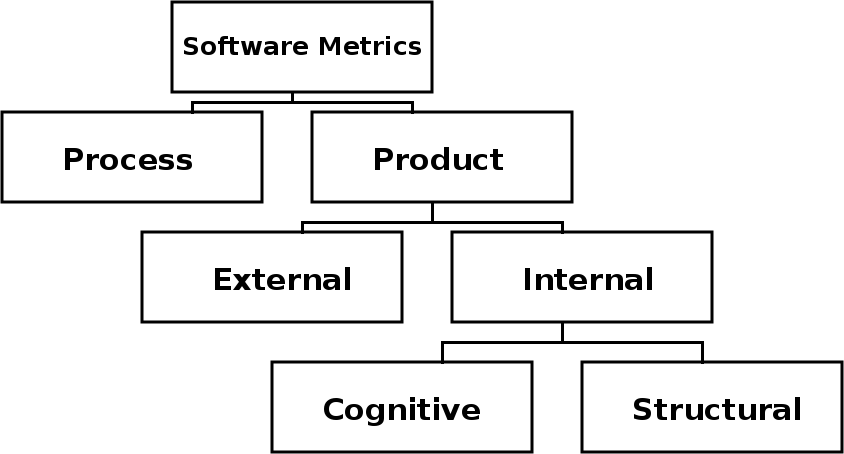
\includegraphics[height=55mm]{figures/classification.png}
	\caption{Classification of software metrics.}
	\label{fig:classification}
\end{figure}

Process metrics are numerical values that depict a software process such as the amount of time require to debug a module~\cite{metrics2}. They are measures of the software development process, such as: overall development time and type of methodology used. Process metrics are collected across all projects and over long periods of time. Their intent is to provide indicators that lead to longterm software process improvement.

Product metrics are measures of software project and are used to monitor and control the project. These metrics measures the complexity of the software design size of the final program number of pages of documentation produced. They enable a software project manager to:

\begin{itemize}
	\item[--] minimize the development time by making the adjustments necessary to avoid delays
	and potential problems and risks.
	\item[--] assess product quality on an ongoing basis and modify the technical approach to improve
	quality.
\end{itemize}

Product metrics are measures of the software product of any stage of its development,from requirements to installed system. Product metrics may measure: the complexity of the software design, the size of the final program, the number of pages of documentation prodused.
Product metrics can be internal or external. External attributes of an entity can be measured only with respect to how the entity relates with the environment and therefore can be measured only indirectly. For example, reliability, an external attribute of a program, does not depend only on the program itself but also on the compiler, machine and user. Productivity, an external attribute of a person, clearly depends on many factors such as the kind of process and the quality of the software delivered. Internal product metrics can be measured only based on the entity and therefore the measures are direct. For example, size is an internal attribute of any software document.

Internal product metrics are subdivided in two categories: cognitive
complexity metrics and structural complexity metrics. Cognitive complexity metrics measure the effort required by developers to understand a system. They aim at discovering the cause of the complexity, which requires understanding human mental processes and details of the software system under development. Structural complexity metrics use the interactions within and among modules to measure a system’s complexity. One of the oldest and most commonly used structural complexity metrics is the number of source lines of code.

Another classification of software metrics is as follows:

\begin{enumerate}
	\item Objective metrics.
	\item Subjective metrics
\end{enumerate}

Objective metrics always results in identical values for a given metric as measured by two or more qualified observers. Whereas subjective metrics are those that even qualified observers may measure different values for a given metric since their subjective judgment is involved in arriving at the measured value.
%%____________________________________________________________________________

\section{Types Of Software Metrics}

It is now apparent that software metrics are important in software
engineering. Symons stated that "a reliable and credible method
for measuring the software development cycle is needed that has a reasonable
theoretica1 basis and that produces results that practitioners can trus" Hence,software metrics have been used to measure a wide range of software
engineering activities.

\subsection{Size-Oriented metrics}

Size-oriented metrics are used to analyze the quality of software.

\textbf{Lines of Code (LOC)}

Lines Of Code (also known as Source Lines of Code - SLOC) is a metric generally used to
evaluate a software program or codebase according to its size. It shows how many lines of source
code there is in the application, namespace, class or method. LoC can be used to: check the size
of code units and estimate the size of project. LOC is the popular and simplest one.
There are two major types of SLOC measures: 

\begin{description}
	\item[Physical SLOC (LOC)] Physical SLOC is a count of lines in the text of the program's source code including comment.
	\item[Logical SLOC(LLOC)] Logical LOC attempts to measure the number of "statements", but their specific definitions are tied to specific computer languages.
\end{description}

Physical SLOC measures are sensitive to logically irrelevant formatting and style conventions, while logical LOC is less sensitive to formatting and style conventions. Unfortunately, SLOC measures are often stated without giving their definition, and logical LOC can often be significantly different from physical SLOC.

\subsection{Object Oriented metrics (OO)}

Chidamber and Kemerer have specified a several metrics for object oriented
designs. All of these metrics are referred to the separate class but not to the whole system.

\textbf{Number Of Methods (NOM)}

The Number Of Methods metric is used to calculate the average count of all class operations per class. A class must have some, but not an excessive number of operations.This information is useful when identifying a lack of primitiveness in class operations (inhibiting
re-use), and in classes which are little more than data types.

\textbf{Number Of Children (NOC)}

NOC is a number of immediate subclasses subordinated to a class in the class hierarchy. NOC counts the number of subclasses belonging to a class.

NOC measures the breadth of a class hierarchy, where maximum DIT measures the depth. Depth is generally better than breadth, since it promotes reuse of methods through inheritance. NOC and DIT are closely related. Inheritance levels can be added to increase the depth and reduce the breadth.

A high NOC, a large number of child classes, can indicate several things: 
\begin{itemize}
	\item High reuse of base class. Inheritance is a form of reuse.
	\item Base class may require more testing.
	\item Improper abstraction of the parent class. 
	\item Misuse of sub-classing. In such a case, it may be necessary to group related classes and introduce another level of inheritance.
\end{itemize}

A class with a high NOC and a high WMC indicates complexity at the top of the class hierarchy. The class is potentially influencing a large number of descendant classes. This can be a sign of poor design. A redesign may be required.

Not all classes should have the same number of sub-classes. Classes higher up in the hierarchy should have more sub-classes then those lower down.


\textbf{Weighted Methods per Class (WMC)}

This metric is the sum of complexities of methods defined in a class. It therefore represents the
complexity of a class as a whole and this measure can be used to indicate the development and
maintenance effort for the class. Classes with a large Weighted Methods Per Class value can often be refactored into two or more classes.

\textbf{Coupling Between Object classes (CBO)}

CBO classes metric represents the number of classes coupled to a given class. This coupling can happen throuhg:
\begin{itemize}
	\item Method call. 
	\item Class extends.
	\item Properties or parameters. 
	\item Method arguments or return types.
	\item Variables in methods
\end{itemize}

Coupling between classes is required for a system to do useful work, but excessive coupling makes the system more difficult to maitain and reuse.At project or package level, this metric provides the average number of classes used per class.

\textbf{Depth of Inheritance Tree (DIT)}

Depth of Inheritance Tree (DIT) is the maximum length of a path from a class to a root class in the inheritance structure of a system. DIT measures how many super-classes can affect a class. DIT is only applicable to object-oriented systems.

The deeper a class is in the hierarchy, the more methods and variables it is likely to inherit, making it more complex. Deep trees as such indicate greater design complexity. Inheritance is a tool to manage complexity, really, not to not increase it. As a positive factor, deep trees promote reuse because of method inheritance.

C\&K suggested the following consequences based on the depth of inheritance:
\begin{itemize}
	\item The deeper a class is in the hierarchy, the greater the number of methods it is likely to inherit, making it more complex to predict its behavior
	\item Deeper trees constitute greater design complexity, since more methods and classes are involved
	\item The deeper a particular class is in the hierarchy, the greater the potential reuse of inherited methods 
\end{itemize}

\textbf{Response For a Class (RFC)} 
The Response for Class (RFC) metric is the total number of methods that can potentially be executed in response to a message received by an object of a class. This number is the sum of the methods of the class, and all distinct methods are invoked directly within the class methods. Additionally, inherited
methods are counted, but overridden methods are not, because only one method of a particular signature will always be available to an object of a given class.

A large RFC has been found to indicate more faults. Classes with a high RFC are more complex and harder to understand. Testing and debugging is complicated. A worst case value for possible responses will assist in appropriate allocation of testing time.
%%___________________________________________________
\subsection{Complexity metrics}
Complexity is an important aspect for software quality assessment and must be appropriately addressed in service-oriented architecture\cite{complexity}.
Cyclomatic complexity one of the most difficult software metrics for understanding.

\textbf{McCabe's Cyclomatic Complexity (MVG)}

McCabe's cyclomatic complexity is a software quality metric that quantifies the complexity of a software program. Complexity is inferred by measuring the number of linearly independent paths through the program. The higher the number the more complex the code.

A pragmatic approximation to this can be found by counting language keywords and operators which introduce extra decision outcomes.
%%_______________________________
\subsection{Structural Metrics}

\textbf{Fan-In and Fan-Out metrics (FIN and FOUT)}

It's a structural metrics which measures inter-module complexities. 
\begin{description}
	\item[Fan-in] Is the number of modules that call a given module.
	\item[Fan-out] Is the number of modules that are called by a given module.
\end{description}

Fan-in and fan-out metrics reflect structure dependency~\cite{fanin}.
This structural metrics were first defined by Henry.
This metrics can be applied both at module level and function level. This metrics just puts a number on how complex is interlinking of different modules or functions. Unlike Cyclomatic complexity you cannot put a number and say it cannot go beyond this number. This is used just to size up how
difficult it will be to replace a function or module in your application and how changes to a function or module can impact other functions or modules. Sometimes you can put restriction on number of Fan-Out a function has to avoid cluttering your function but is not a widely accepted practice.

%%______________________________________________________

\subsection{Cohesion metrics}
Cohesion is an important software quality attribute and high cohesion is one of characteristics of well-structured software design~\cite{cohesion}.
Cohesion metrics analyze the connection between methods of a class.
Module cohesion indicates relatedness in the functionality of a software module~\cite{cohesion2}.

\textbf{Lack of Cohesion in Methods (LCOM)}

LCOM measures the amount of cohesiveness present, how well a system has been designed and how complex a class is. LCOM is a count of the number of method pairs whose similarity is zero,minus the count of method pairs whose similarity is not zero. LCOM is probably the most controversial and argued over of the C\&K metrics.

C\&K's rationale for the LCOM method was as follows:
\begin{itemize}
	\item Cohesiveness of methods within a class is desirable, since it promotes encapsulation.
	\item Lack of cohesion implies classes should probably be split into two or more subclasses.
	\item Any measure of disparateness of methods helps identify flaws in the design of classes. 
	\item Low cohesion increases complexity, thereby increasing the likelihood of errors during the development process.
\end{itemize}

Although there is a fair amount of debate about how to calculate LCOM and it features in a lot of metrics sets an increasing number of researchers suggest that it is not a particularly useful metric. Perhaps this is also reflected in there being a fair amount of debate about how to calculate LCOM but very little on how to interpret it and how it fits in with other metrics. 

\textbf{Tight and Loose Class Cohesion (TCC and LCC)}

TCC(Tight Class Cohesion) and LCC(Loose Class Cohesion) metrics measure  the  relative number of directly-connected pairs of methods and the   relative   number of directly- or indirectly- connected pairs of methods.
The Tight Class Cohesion metric measures the cohesion between the public methods of a class. That is the relative number of directly connected public methods in the class. Classes having a low cohesion indicate errors in the design.

TCC considers two methods to be connected if they share the  use  of  at  least  one  attribute.  A  method  uses  an  attribute if the attribute appears in the method’s body or  the  method  invokes  directly  or  indirectly  another method   that   has   the   attribute   in   its   body.   
The higher TCC and LCC, the more cohesive and thus better the class.


%%______________________________________________________________________

\section{Software Metric Tools}
There are number of software metrics have been developed and numerous tools exist to collect the metrics from program representations. This large variety of tools allows a user to select the tool best suited as per the use requirements for example it's handling, tool support ,cost etc. This is assumed that the metrics computed by the metric tools are same for all the metric tools. One can think of a software metric tool as a program which implements a set of software metrics definitions. It allows to access a software system according to the metrics by extracting the required entities from the software ad providing the corresponding metric values. There are
some criteria for selecting the proper metric tools as the availability of the software tools can make confusion. One such criterion is that the tools must have to calculate any form of software metrics. Majority metric tools are available for Java programs. Many tools are just code counting
tool, they basically count the variants of the lines of code(LOC) metric. The specific criteria areas follows language: Java(source or byte code), metrics: well known object oriented metrics on class level, license: freely available.

\subsection{CCCC}

It is a little command-line tool that generates metrics from the source code of a C or C++ project. The output of the tool is a simple HTML website with information about all your sources. It generates reports on various metrics including lines of code (LOC) and metrics proposed by Chidamber\&Kemererand Henry\&Kafura. CCCC has been developed as freeware, and is released in source code form. Users are encouraged to compile the program themselves, and to modify the source to reflect their preferences and interests.

CCCC will process each of the files specified on the command line (using standard wildcard processing were appropriate. For each file, named, CCCC will examine the extension of the filename, and if the extension is recognized as indicating a supported language, the appropriate parser will run on the file. As each file is parsed, recognition of certain constructs will cause records to be written into an internal database. When all files have been processed, a report on the contents of the internal database
will be generated in HTML format. By default the main summary HTML report is generated to the file cccc.htm in a subdirectory called .cccc of the the current working directory, with detailed reports on each module (i.e. C++ or Java class) identified by the analysis run).

In addition to the summary and detailed HTML reports, the run will cause generation of corresponding summary and detailed reports in XML format, and a further file called cccc.db to be created. cccc.db will contain a dump of the internal database of the program in a format delimited with the character '@' (chosen because it is one of the few characters which cannot legally appear in C/C++ non -comment source code).

The report contains a number of tables identifying the modules in the files submitted and covering:
\begin{enumerate}
	\item Measures of the procedural volume and complexity of each module and its functions;. 
	\item Measures of the number and type of the relationships each module is a party to either as a client or a supplier.
	\item Identification of any parts of the source code submitted which the program failed to parse.
	\item A summary report over the whole body of code processed of the measures identified above.
\end{enumerate}

This tool can measure the following metrics:
\begin{itemize}
	\item Lines of Code (LOC). 
	\item Weighted Methods per Class(WMC).
	\item Fan-In Fan-Out()FIN and FOUT).
	\item Numbe r Of Children(NOC).
	\item Number Of Methods (NOM).
	\item McCabe's Cyclomatic Complexity(MVG).
\end{itemize}

\subsection{Chidamber\&Kemerer}

The program calculates Chidamber and Kemerer object-oriented metrics by processing the bytecode of compiled Java files.It is open source command line tool. The program calculates for each class the following six metrics, and displays them on its standard output, following the class's name.

This tool can measure the following metrics:

\begin{itemize}
	\item Weighted Methods per Class(WMC).
	\item Depth of Inheritance Tree (DIT).
	\item Coupling Between Object classes (CBO).
	\item Numbe r Of Children(NOC).
	\item Response For a Class (RFC).
	\item Lack of Cohesion in Methods (LCOM).
\end{itemize}

\subsection{Analyst4j}
It is based on the Eclipse platform and available as a standalone Rich Client Applications or as an Eclipse
IDE plug in. It features search, metrics,analyzing quality,report generating for Java programming.
Analyst4j tool are most popular to findout the quality related metrics. This tool is based on Chidamber\&Kemerer metrics.

This tool can measure the following metrics:
\begin{itemize}
	\item Lines of Code (LOC). 
	\item Weighted Methods per Class(WMC).
	\item Depth of Inheritance Tree (DIT).
	\item Coupling Between Object classes (CBO).
	\item Numbe r Of Children(NOC).
	\item Response For a Class (RFC).
	\item Number Of Methods (NOM).
	\item Lack of Cohesion in Methods (LCOM).
\end{itemize}

\subsection{OOMeter}

OOMeter is a software metric tool for measuring the quality attributes of Java and C\# source code and UML models, stored in XMI format. OOMeter has a rich collection of object-oriented software metrics. It is an Eclipse plug in. It provides an SQL like querying language for object-oriented code which
allows to search for bugs, measure code metrics etc.

OOMeter provides an interface for users to define custom metrics through java classes that implement a certain interface. It supports export of metric results to a number of formats, including XML, HTML, delimited text, Microsoft Excel, etc.

This tool can measure the following metrics:

\begin{itemize}
	\item Lines of Code (LOC). 
	\item Weighted Methods per Class(WMC).
	\item Depth of Inheritance Tree (DIT).
	\item Coupling Between Object classes (CBO).
	\item Numbe r Of Children(NOC).
	\item Response For a Class (RFC).
	\item Lack of Cohesion in Methods (LCOM).
	\item Tight Class Cohesion (TCC).
\end{itemize}



\subsection{Eclipse Metrics plugin 1.3.6}

This  is an open source metrics calculation and dependency analyzer a  metrics plugin for Eclipse IDE. The plugin is also provided 
integrated  as  an  EasyEclipse  package.  The  plugin computes   the  various metrics and displays it in the integrated view.


This tool can measure the following metrics:

\begin{itemize}
	\item Lines of Code (LOC). 
	\item Weighted Methods per Class(WMC).
	\item Depth of Inheritance Tree (DIT).
 	\item Numbe r Of Children(NOC).
    \item Number Of Methods (NOM).
\end{itemize}

\subsection{Eclipse Metrics plugin 3.4}
The  eclipse  plugin  3.4 developed  by  Lance  Walton  is  also  integrated  with Eclipse   and   is   available   for   all   Java   projects 
developed using the ID.E It is a open source tool. It calculates various metrics during build cycles and warns via the problem view of metrics range violations.

This tool can measure the following metrics:
\begin{itemize}
	\item Lines of Code (LOC). 
	\item Weighted Methods per Class(WMC).
	\item Depth of Inheritance Tree (DIT).
    \item Lack of Cohesion in Methods (LCOM).
\end{itemize}

\subsection{Semmle}

Semmle is an analysis platform that produces detailed analyses of the code base for one or more software projects. For each project that it analyzes, it measures artifacts against rules that check for good practice. Analysis is scheduled to occur on a regular basis. As part of this process a copy of the source code is checked out of the repository for analysis. The code, and related artifacts, is checked against rules, defined using queries, to identify any alerts. In addition, metrics are calculated and data may be imported from third-party systems used by your company. A database is created, containing detailed information about the artifacts and each alert.

This tool can measure the following metrics:
\begin{itemize}
	\item Depth of Inheritance Tree (DIT).
	\item Lack of Cohesion in Methods (LCOM).
	\item Numbe r Of Children(NOC).
	\item Number Of Methods (NOM).
	\item Response For a Class (RFC).
\end{itemize}

\section{Measuring functional languages}
In previous section has been described sofrware metrics for object-oriented languages. However software metrics developed for imperative and object-oriented languages can also be used for measuring in functional programming languages like Erlang and Haskell. We can use the same metrics because several constructs as a class,  a module and a library are similar. All of this structures can be consider like collections of functions. If the chosen metric does not take the distinctive properties of these constructs into account (variables, method overrides, dynamic binding, visibility etc.), then it can be applied to these apparently diverse constructs ~\cite{metrics3}.

Dissimilarity between functional and imperative languages are in such features as difference in the level of nesting of blocks and control
structures, in several ways of connecting certain functions (for example, data flow and call graph), inheritance insted of cohesion and and simple cardinality metrics(lines of code, char of code).


Another difference functional programming languages from imperative languages is there are some constructs and properties that can be used only in functional programming languages as: list comprehensions, pattern matching, referential transparency of pure functions, currying, laziness of expression evaluation.

While these features raise the expressive power of functional languages,
most of the existing complexity metrics require some changes before they be-
come applicable to functional languages ~\cite{metrics3}.

There are general metrics are acceptable for functional languages:
\begin{itemize}
	\item \textbf{Branches of recursion}.This metric allows to measure how many times did the function call itself
	\item \textbf{Fun expressions and message passing constructs}.
	\item \textbf{Return points of a function}.
	\item There is possible to calculate metrics on a single clause of a function.
	\item There is possible to calculate metrics on a single clause of a function.
	\item \textbf{Otp used}. This metric allows measure OTP behaviours.
\end{itemize}

In the next chapter will be described all developed metrics for Erlang in details.





\chapter{Software metrics in Erlang}
In this chapter, we present a developed framework which allows to analyze Erlang programs and visualize calculated metrics. The first two sections give a brief summary of Erlang, RefactorErl static analysis tool and developed metrics.

\section{An introductory glimpse at the Erlang programming language}
Erlang is a functional programming language which provides runtime designed for highly parallel, scalable software requiring high uptime. It is designed for development of robust systems that can be distributed between many different computers in a network. Erlang is kinda of similar to Java in the case that it uses a virtual machine and also supports multithreading. 

\textbf{Variables}
Erlang provides dynamic data types, allowing programmers to develop system
components (such as message dispatchers) that do not care what type of data they are handling and others that strongly enforce data type restrictions or that decide how to act based on the type of data they receive. Variables must start with a capital letter or an underscore, and are composed of letters, digits,	 and underscores.

\textbf{Data types}
Erlang has:
\begin{enumerate}
	\item Integers of unlimited size.
	\item Floats.
	\item Strings, placed within double quotes: "It is some string.".
	\item Atoms. An atom is an element by itself. It starts with a lowercase letter and is built of letters, digits, and underscores, or it is any string placed within single quotes: atom1, 'Atom 2'.
	\item Lists are a comma-separated sequence of some values placed within brackets: [abc, 123, "It is some string"]. 
	\item Tuples are a comma-separated sequence of some values placed within braces: \{abc, 123, "It is some string"\}.
	\item Records are not a separate data type but are just tuples with keys associated with each value. They are declared in a file and defined (given specific values) in the program.
	\item Binaries are placed within double angle brackets: <<0, 128, 128, 255>>, <<"It is some string">>, <<X:7, Y:5, Z:1>>. Binaries are series of bits; the number of bits in a binary has to be a multiple of 8.
	\item References are globally unique values.
	\item Pids stand for process identifiers.
\end{enumerate}

Figure \ref{fig:example_erlang} features the source of a small Erlang program
called example that demonstrated recursive list manipulation.
\begin{figure}[ht]
	\begin{lstlisting}[extendedchars=true, language=Erlang, basicstyle=\footnotesize\ttfamily, keywordstyle=\color{red}]
	-module(example). 
	-export([max/1, min/1, sum/1]).
	
	%% Find the maximum of a list.
	max([H|T]) -> max2(T, H).
	max2([], Max) -> Max;
	max2([H|T], Max) when H > Max -> max2(T, H);
	max2([_|T], Max) -> max2(T, Max).
	

	%% Find the minimum of a list.
	min([H|T]) -> min2(T,H).
	min2([], Min) -> Min;
	min2([H|T], Min) when H < Min -> min2(T,H);
	min2([_|T], Min) -> min2(T, Min).
	
	%% Find the sum of all the elements of a list.
	sum(L) -> sum(L,0).
	sum([], Sum) -> Sum;
	sum([H|T], Sum) -> sum(T, H+Sum).
	\end{lstlisting}
\caption{A simple module in Erlang.}
\label{fig:example_erlang}
\end{figure}

Erlang source files consist of a section containing meta-information about the module represented by the file (all functions in Erlang must be defined in
modules.), and a list of functions that are either exposed to the users of this module (with the -export attribute), or are only defined for internal use inside the module.  

A subtle element of all three functions is that every function needs to have an initial value to start counting with. In the case of \texttt{sum/2}, we use 0, as we’re doing addition, and given \texttt{X = X + 0}, the value is neutral, so we can’t mess up the calculation by starting there. If we were doing multiplication, we would use 1 given \texttt{X = X * 1}. 

The functions \texttt{min/1} and \texttt{max/1} can’t have a default starting value. If the list were only negative numbers and we started at 0, the answer would be wrong. So we need to use the first element of the list as a starting point.

\section{The RefactorErl static analysis tool} 

RefactorErl ~\cite{refactorerl1, refactorerl2} is an open-source static source code analyzer and transformer tool for Erlang, developed by the Department of Programming Languages and Compilers at the Faculty of Informatics, Eötvös Loránd University, Budapest, Hungary. The phrase "refactoring" means a preserving source code transformation, so while you change the program structure you do not alter its behavior. RefactorErl was built to refactor Erlang programs.

The main focus of RefactorErl is to support daily code comprehension tasks of Erlang developers ~\cite{refactorerl}. It can analyze the structure of the refactored program - based on the syntactic rules of the underlying programming language - and it can also collect and use semantical information about the source code.

\subsection{Metrics in the RefactorErl}

A metric query language is incorporated into RefactorErl ~\cite{refactorerlimp}. Metric queries can be executed from the console interface or can be used as properties in semantic query language which is available from every interface.

Table \ref{tab:metrics_ref} shows all the implemented metrics in RefactorErl tool. There are two columns in this table: the first column gives the information about the name of the metric, and the second column shows the for which node the metric is available.

\begin{table}[!htb]
	\centering
	\caption{Implemented metrics in RefactorErl}
	\label{tab:metrics_ref}
	\noindent\adjustbox{max width=0.9\textwidth}{
		\begin{tabular}{|c|c|}
			\hline
			\textbf{Name of the metric}  & \textbf{Node type} 
			\\
			\hline
			module sum					& module
			\\
			
			\hline
			line of code				& module/function
			\\
			
			\hline
			char of code				& module/function
			\\
			
			\hline
			number of fun				& module
			\\
			
			\hline
			number of macros			& module
			\\
			
			\hline
			number of records			& module
			\\
			
		  	\hline
			included files				& module
			\\	
				
		  	\hline
		  	imported modules			& module
		  	\\	
		  	
		  	\hline	
		  	number of funpath			& module
		  	\\	

		  	\hline
		  	function calls in			& module
		  	\\
		  	
		  	\hline
		  	function calls out			& module
		  	\\	
		  	
		  	\hline
		  	cohesion					& module
		  	\\	  	
		  	
		  	\hline
		  	function sum				& function
		  	\\	  	
		  			  	
		  	\hline
		  	max depth of calling		& module/function		  			  
		  	\\
		  	
		  	\hline
		  	max depth of cases			& module/function		  			  
		  	\\		
		  	  	
		  	\hline
		  	min depth of cases			& module/function		  			  
		  	\\		  	

		  	\hline
		  	max depth of structs		& module/function		  			  
		  	\\		  			

		  	\hline
		  	number of funclauses		& module/function		  			  
		  	\\			
	
		  	\hline
		  	branches of recursion		& module/function		  			  
		  	\\			

		  	\hline
		  	calls for function			& function		  			  
		  	\\			
			
		  	\hline
		  	calls from function			& function		  			  
		  	\\	

		  	\hline
		  	number of funexpr			& module/function		  			  
		  	\\
		  	
		  	\hline
		  	number of messpass			& module/function		  			  
		  	\\		  	

		  	\hline
		  	fun return points			& module/function		  			  
		  	\\	
		  	
		  	\hline
		  	average size				& module/function		  			  
		  	\\		  		  	

		  	\hline
		  	max length of line			& module/function		  			  
		  	\\
		  	
		  	\hline
		  	no space after comma		& module/function		  			  
		  	\\	
		  	
		  	\hline
		  	is tail recursive			& function		  			  
		  	\\		  	

		  	\hline
		  	mcCabe						& module/function		  			  
		  	\\	
		  			  	
		  	\hline
		  	otp used						& module		  			  
		  	\\			  	
		  	\hline		  		  			  				
		\end{tabular}}
	\end{table}

\textbf{module\_sum}

The sum of the chosen complexity structure metrics measured on the functions of the module. The proper metrics adjusted in a list can be implemented in the desired number and order ~\cite{refactorerlm}.

\textbf{line\_of\_code}

The number of lines of part of the text, function, or module. The number of empty lines is not included in the sum. As the number of lines can be measured on more functions, or modules and the system is capable of returning the sum of these, the number of lines of the whole loaded program text can be enquired ~\cite{refactorerlm}.

\textbf{char\_of\_code}

The number of characters in a program script. This metric is capable of measuring both the codes of functions and modules and with the help of aggregating functions we can enquire the total and the average number of characters in a cluster, or in the whole source text ~\cite{refactorerlm}.

\textbf{number\_of\_fun}

This metric gives the number of functions implemented in the concrete module, but it does not contain the number of non-defined functions in the module~ \cite{refactorerlm}.

\textbf{number\_of\_macros}

This metric gives the number of defined macros in the concrete module or modules. It is also possible to inquire the number of implemented macros in a module ~\cite{refactorerlm}.

\textbf{number\_of\_records}

 This metric gives the number of defined records in a module. It is also possible to inquire the number of implemented records in a module ~\cite{refactorerlm}.

\textbf{included\_files}

This metric gives the number of visible header files in a module ~\cite{refactorerlm}.

\textbf{imported\_modules}

This metric gives the number of imported modules used in a concrete module. The metric does not contain the number of qualified calls (calls that have the following form: module:function) ~\cite{refactorerlm}.

\textbf{number\_of\_funpath}

The total number of function paths in a module. The metric, besides the number of internal function links, also contains the number of external paths or the number of paths that lead outward from the module. It is very similar to the metric called cohesion ~\cite{refactorerlm}.

\textbf{function\_calls\_in}

Gives the number of function calls into a module from other modules. It can not be implemented to measure a concrete function. For that, we use the calls\_for/1 function ~\cite{refactorerlm}.

\textbf{function\_calls\_out}

Gives the number of every function call from a module towards other modules. It can not be implemented to measure a concrete function. For that, we use the calls\_from/1 function ~\cite{refactorerlm}.

\textbf{cohesion}

The number of call-paths of functions that call each other. By call-path we mean that an f1 function calls f2 (e.g. f1()->f2().). If f2 also calls f1, then the two calls still count as one call-path ~\cite{refactorerlm}.

\textbf{function\_sum}

The sum calculated from the functions complexity metrics characterizes the complexity of the function. It can be calculated using various metrics together ~\cite{refactorerlm}.
	 
\textbf{max\_depth\_of\_calling}

The length of function call-chains, namely the chain with the maximum depth ~\cite{refactorerlm}.
	 
\textbf{max\_depth\_of\_cases}

 Gives the maximum of case control structures embedded in case of a concrete function (how deeply are the case control structures embedded). In case of a module, it measures the same regarding all the functions in the module. Measuring does not break in case of case expressions, namely when the case is not embedded ~\cite{refactorerlm}.

\textbf{min\_depth\_of\_cases}

 Gives the minimum of the maximums of case control structures embedded in case of a concrete function (how deeply are the case control structures embedded). In case of a module it measures the same regarding all the functions in the module. Measuring does not break in case of case expressions, namely when the case is not embedded into a case structure. However, the following embedding does not increase the sum ~\cite{refactorerlm}.

\textbf{max\_depth\_of\_structs}

 Gives the maximum of structures embedded in function (how deeply are the block, case, fun, if, receive, try control structures embedded). In case of a module it measures the same regarding all the functions in the module ~\cite{refactorerlm}.

\textbf{number\_of\_funclauses}

Gives the number of functions clauses. Counts all distinct branches, but does not add the functions having the same name, but different arity, to the sum ~\cite{refactorerlm}.

\textbf{branches\_of\_recursion}

Gives the number of branches of a certain function, how many times a function calls itself, and not the number of clauses it has besides definition ~\cite{refactorerlm}.

\textbf{calls\_for\_function}

This metric gives the number of calls for a concrete function. It is not equivalent to the number of other functions calling the function, because all of these other functions can refer to the measured one more than once ~\cite{refactorerlm}.

\textbf{calls\_from\_function}

This metric gives the number of calls from a certain function, namely how many times does a function refer to another one (the result includes recursive calls as well) ~\cite{refactorerlm}.

\textbf{number\_of\_funexpr}

Gives the number of function expressions in a module. It does not measure the call of function expressions, only their initiation ~\cite{refactorerlm}.

\textbf{number\_of\_messpass}

In the case of functions, it measures the number of code snippets implementing messages from a function, while in case of modules it measures the total number of messages in all of the modules functions ~\cite{refactorerlm}.

\textbf{fun\_return\_points}

The metric gives the number of the functions possible return points (or the functions of the given module) ~\cite{refactorerlm}.

\textbf{average\_size}

The average value of the given complexity metrics (e.g. Average branches\_of\_recursion calculated from the functions of the given module) ~\cite{refactorerlm}.

\textbf{max\_length\_of\_line}

It gives the length of the longest line of the given module or function ~\cite{refactorerlm}.

\textbf{average\_length\_of\_line}

It gives the average length of the lines within the given module or function ~\cite{refactorerlm}.

\textbf{no\_space\_afte\r\_comma}

It gives the number of cases when there are not any whitespaces after a comma or a semicolon in the text of the given module or function ~\cite{refactorerlm}.

\textbf{is\_tail\_recursive}

It returns with 1 if the given function is tail recursive; with 0, if it is recursive, but not tail recursive; and -1 if it is not a recursive function (direct and indirect recursions are also examined). If we use this metric from the semantic query language, the result is converted to tail\_rec, non\_tail\_rec or non\_rec atom ~\cite{refactorerlm}.

\textbf{mcCabe}

McCabe cyclomatic complexity metric. We define it based on the control flow graph of the functions with the number of different execution paths of a function, namely the number of different outputs of the function ~\cite{refactorerlm}.

\textbf{otp\_used}

Gives the number of OTP callback modules used in modules ~\cite{refactorerlm}.

\section{Metric visualisation module for WEB2 interface of RefactorErl}

The section describes the main concept and details of the developed framework for RefactorErl static analysis tool. The first part introduces the main features of the software. The next part describes which tools were used in the developing process of the module. In the last part, we can read how to use the software step-by-step.

\subsection{Description of the software}

The program which was developed allows analyzing git repositories with Erlang code files. The component is built on RefactorErl static analysis tool and actively uses its feature of calculating different metrics of Erlang modules and functions. It has convenient user-friendly web interface with repository structure as a folder tree and a canvas where plots can be observed. These plots contain information how particular metric was changing with repository evolution. The plot can be saved for future use as a picture in PNG format.

The main features of the software are:
\begin{itemize}
	\item Drawing plots which show the change of metrics with software evolving from version to version.
	\item Analyzing modules and functions separately.
	\item Choosing separate files for the analyzing.
	\item User-friendly web interface.
\end{itemize}

The main focus of the project is to help Erlang developers with analyzing their projects using plots. Visualization helps with finding patterns and improving the code quality. 

\subsection{Used tools}

The interface of the program is the AngularJS component which uses NVD3 library for plot rendering. Metrics data is stored in DETS tables at the stage of calculation in Erlang code. This data passes as JSON objects when Erlang function communicates with javascript code. For saving plots as pictures the saveSvgAsPng library is used.

\textbf{NVD3}

This library currently under development of a team of software engineers at Novus Partners company ~\cite{nv}. NVD3 is the D3 based JavaScript library. It allows creating beautiful and reusable charts in web applications.

It has wonderful features for data visualization with nice-looking charts such as the usual box-plot, line and bar charts and fancier candlestick and sunburst charts. If you need a lot of functionality in a JavaScript chart plotting library, NVD3 is the very nice option for your project.

\textbf{AngularJs}

The new component was created for the existing system using this javascript web framework.

AngularJS (also written as Angular.js) is an open-source JavaScript-based front-end web application framework mainly developed by Google and by a community of individuals and corporations to solve many of the challenges which can be observed in the development of single-page applications ~\cite{angular}.

The AngularJS framework starts his work by reading the Hypertext Markup Language (HTML) page, which has extra tag attributes embedded into it. Angular transforms these attributes as directives to bind input or output parts of the page to a model that is defined by standard JavaScript variables. The values of these JavaScript variables can be manually set in the code, or fetched from static or dynamic JSON resources. 

\textbf{DETS tables}

Data of calculated metrics for modules and functions stored in two different tables: mods\_metrics and funs\_metrics.

DETS is Disk Erlang Term Storage. DETS tables store tuples, with access to the elements given through a  key field in the tuple. The tables are implemented using hash tables and binary trees, with different representations providing different kinds of collections ~\cite{erlang_o'reilly}.

\textbf{JSON}

Data, which stored in Dets tables, transforms into JSON objects when Erlang code interact with JavaScript code. JSON (JavaScript Object Notation) is a simple format of data-interchange ~\cite{json}. It is a text format that is absolutely language independent but it uses a convention that is familiar to programmers of the C-family of languages which includes C, C++, C\#, Java, JavaScript, Python, Perl, and others. This property makes JSON an ideal language of data-interchange.

JSON is built on two data structures:
\begin{itemize}
	\item Key/value pairs collection. In various languages, this is realized as an object, struct, record, hash table, dictionary, associative array or keyed list ~\cite{json}.
	\item An ordered list of values. Usually, this is realized as an array, list, vector, or sequence ~\cite{json}.
\end{itemize}

\textbf{saveSvgAsPng}

This small library is used for saving SVG plots as PNG pictures ~\cite{saveSvgAsPng}. Despite its small size, it has a lot of different options such a choosing particular background, font, scale etc. 

\subsection{The typical workflow}

For using the component WEB2 interface should be run. It can be done with this command executed in RefactorErl shell:

\begin{lstlisting}[frame=none, numbers=none]
	ri:start_web2([{yaws_path, PATH-TO-YAWS}]).
\end{lstlisting}

This command will run WEB2 interface available on localhost:8001 by default. After loginning the component can be accessed in the metrics tab as shown in Figure \ref{fig:interface}.

\begin{figure}[ht]
	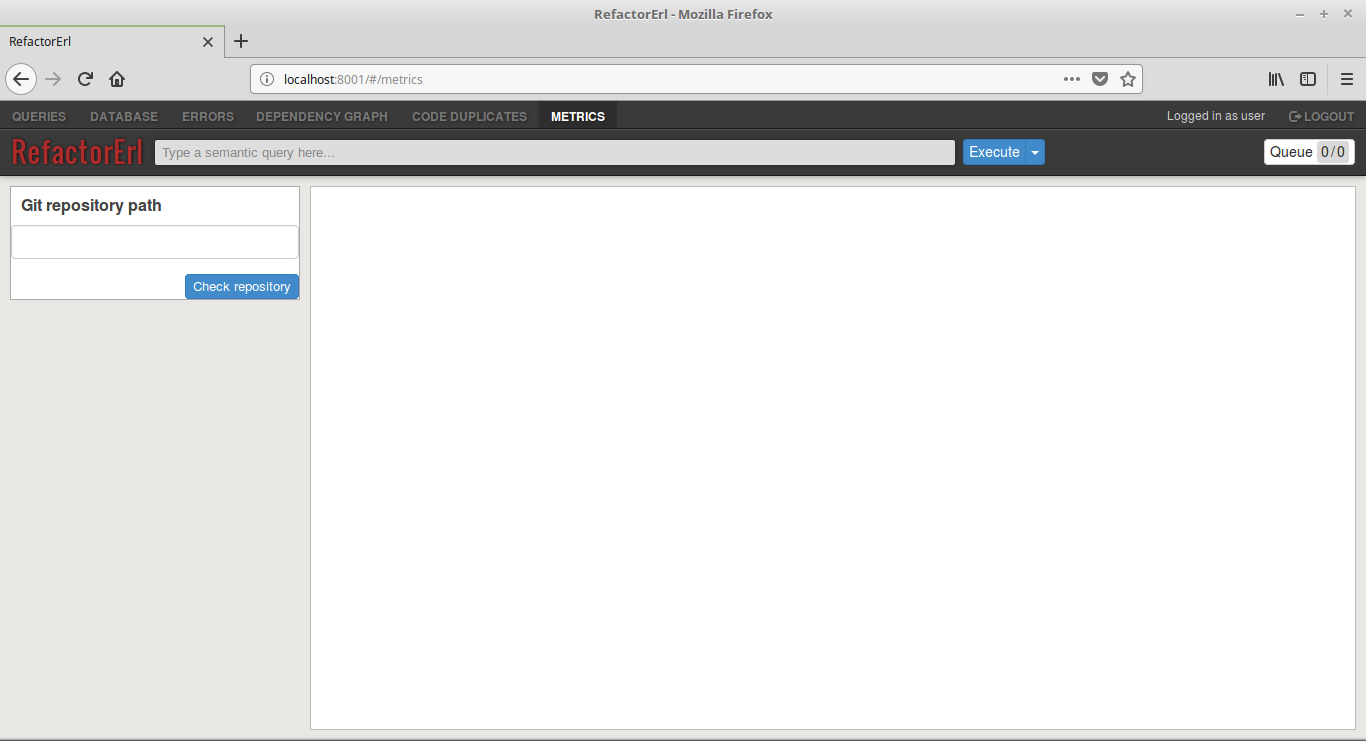
\includegraphics[width=\textwidth]{figures/metrics.png}
	\caption{Component interface.}
	\label{fig:interface}
\end{figure}

The path to git repository should be provided in "Git repository path" input. After clicking the "Check repository" button the folder will be analyzed. If it is not valid the alert Figure \ref{fig:metrics_alert} will be shown.  

\begin{figure}[ht]
	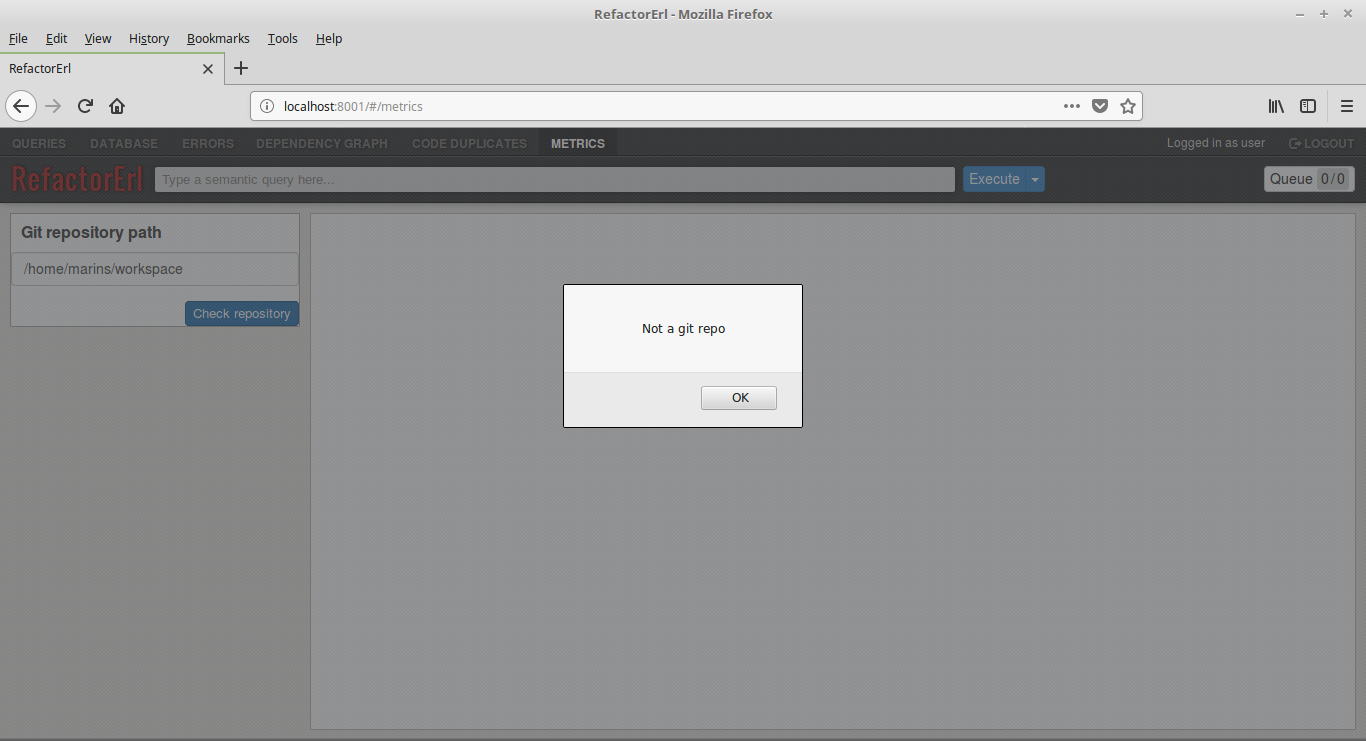
\includegraphics[width=\textwidth]{figures/alert.png}
	\caption{Alert showed because the provided folder is not a valid repository.}
	\label{fig:metrics_alert}
\end{figure}

In another case, the folder tree will be available where separate files can be chosen for future analyzing as shown in Figure \ref{fig:metrics_files}. Also, there is a possibility to delete some files chosen by mistake.

\begin{figure}[ht]
	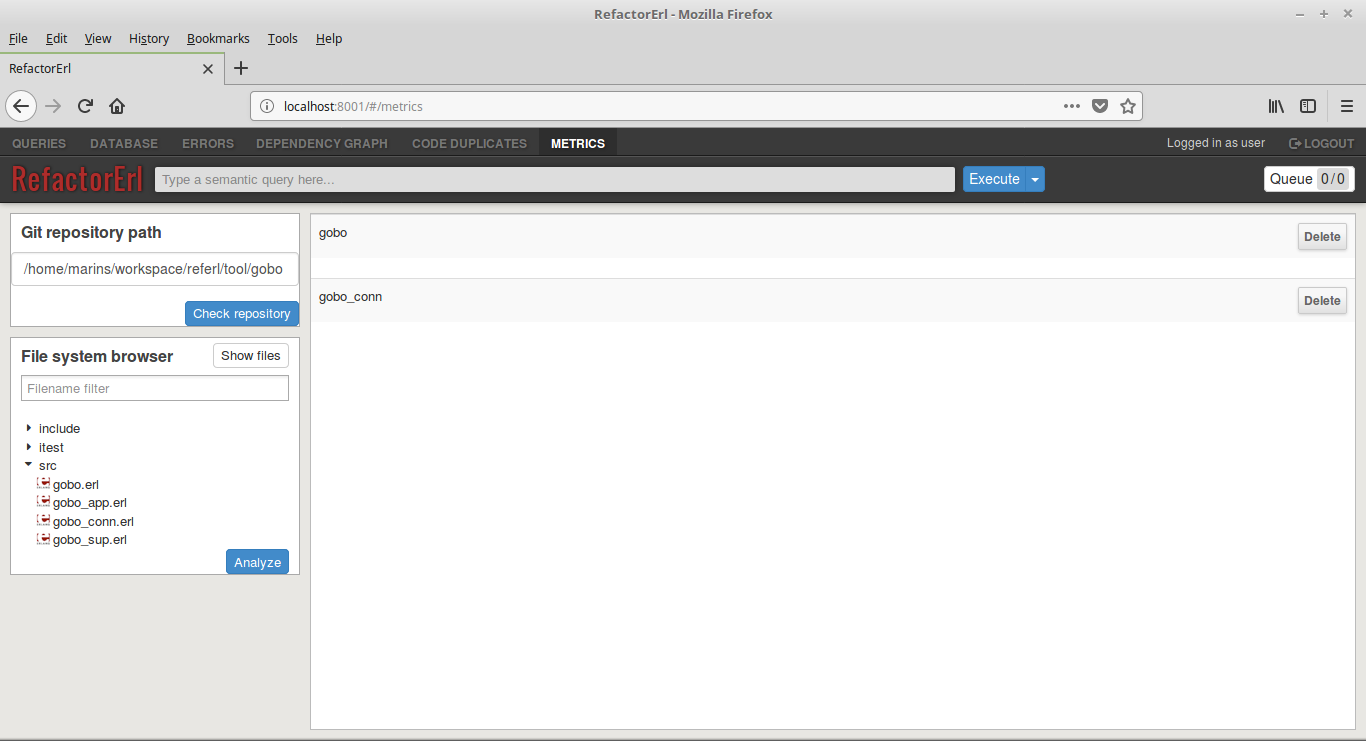
\includegraphics[width=\textwidth]{figures/files.png}
	\caption{Repository tree.}
	\label{fig:metrics_files}
\end{figure}

The final step is pressing the "Analyze" button. It will start calculating metrics for all versions of the repository and progress will be shown on screen Figure \ref{fig:metrics_analyze}. 

\begin{figure}[ht]
	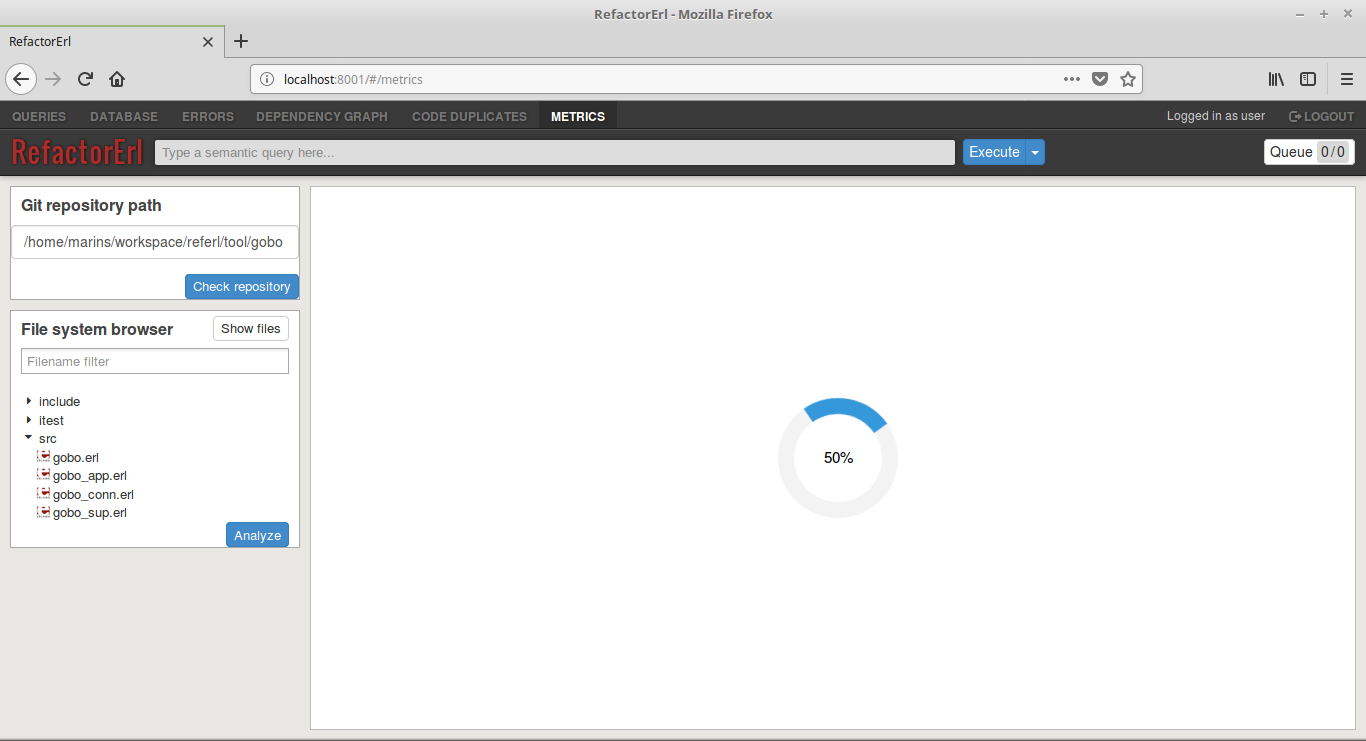
\includegraphics[width=\textwidth]{figures/analyze.png}
	\caption{The process of repository analyzing.}
	\label{fig:metrics_analyze}
\end{figure}

After analysis is done the menu with choosing parameters of drawing the plot will be available as shown at Figure \ref{fig:metrics_plot}. It consists of two selection lists. The first one is the list where we can choose the type of item for plots drawing (module or function). Depends on the chosen type the select boxes with available metrics will differ. 

For modules: module sum, line of code, char of code, number of fun, number of macros, number of records, included files, imported modules, number of funpath, function calls in, function calls out, cohesion, max depth of calling, max depth of cases, min depth of cases, max depth of structs, number of funclauses, branches of recursion, number of funexpr, number of messpass, fun return points, average size, max length of line, no space after comma, mcCabe, otp used.

For functions: line of code, char of code, function sum, max depth of calling, max depth of cases, min depth of cases, max depth of structs, number of funclauses, branches of recursion, calls for function, calls from function, number of funexpr, number of messpass, fun return points, average size, max length of line, no space after comma, is tail recursive, mcCabe. Another list is the list of all items which can be chosen for metrics plot drawing. 

After the plot is shown the "Save" button appears which can be pressed to save SVG plot in a PNG file. 

\begin{figure}[ht]
	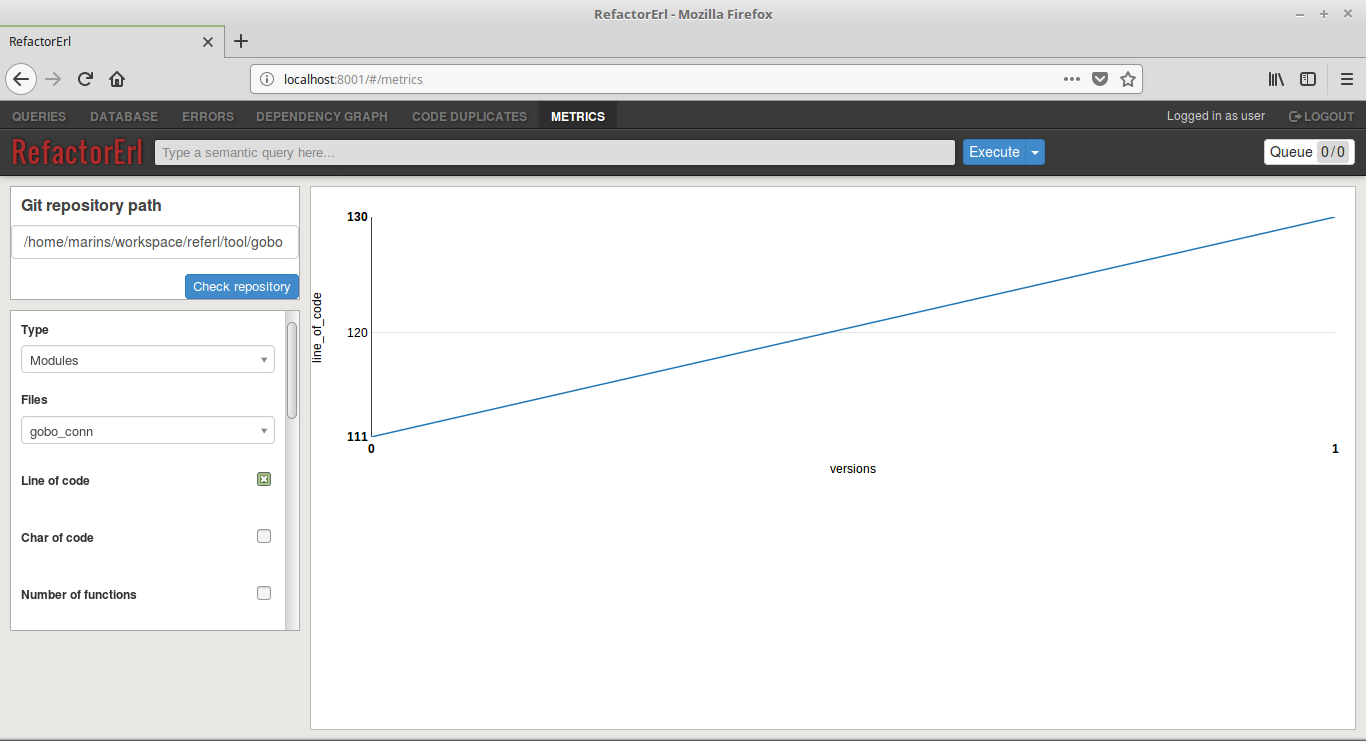
\includegraphics[width=\textwidth]{figures/plot.png}
	\caption{The example of plot.}
	\label{fig:metrics_plot}
\end{figure}

\chapter{Measurements and findings}
The aim of this chapter is to test and analyze projects from git by using the developed module for RefactorErl. Git commit logs hold all the change history. This is an excellent source to observe trends and patterns about projects. All projects selected for the experiment are written in Erlang and have more than 40 commits.

\section{Iron}

This project is functional Erlang Toolkit. Iron is released under the MIT license. It can do the foolowing:
\begin{itemize}
	\item Count with coerce equality, count with a custom predicate.
	\item Find with coerce equality, find with a custom predicate.
\end{itemize}

This project has just only one source code file with 68 commits. The link to the repository is \url{https://github.com/elementerl/iron}.

We can see that with the version number increase the line of code number and char of code number also grow on Figure \ref{fig:loc_iron} and in Figure \ref{fig:char_iron}.

\begin{figure}[ht]
	\centering
	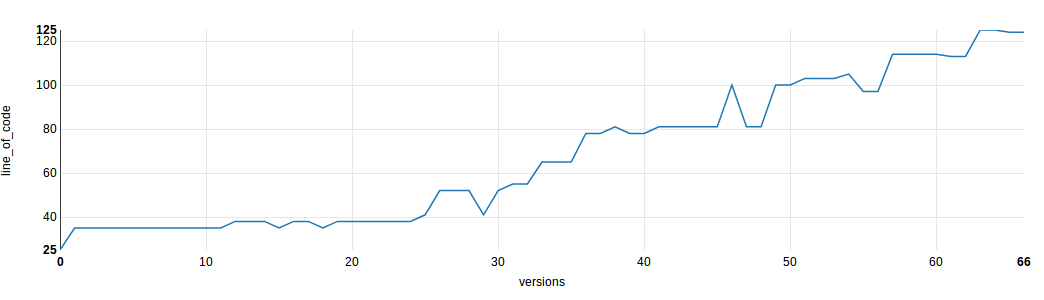
\includegraphics[width=\textwidth]{figures/loc_iron.png}
	\caption{Effective Line of code for fe.erl file.}
	\label{fig:loc_iron}
\end{figure}

\begin{figure}[ht]
	\centering
	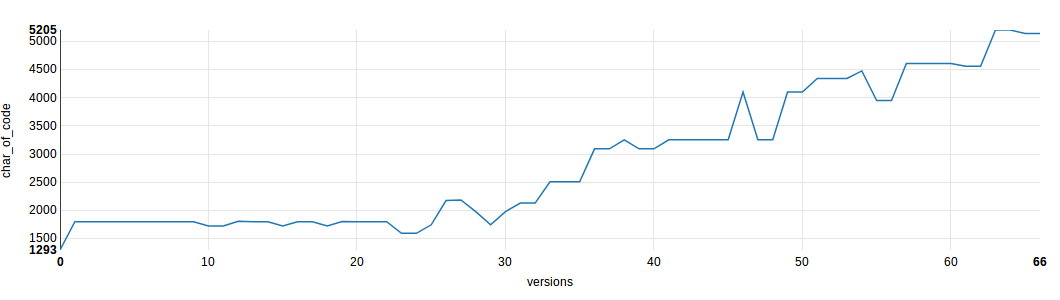
\includegraphics[width=\textwidth]{figures/char_iron.png}
	\caption{Char of code for fe.erl file.}
	\label{fig:char_iron}
\end{figure}

As shown in Figure \ref{fig:otp_iron} developer started to use otp library after 45th version. 

\begin{figure}[ht]
	\centering
	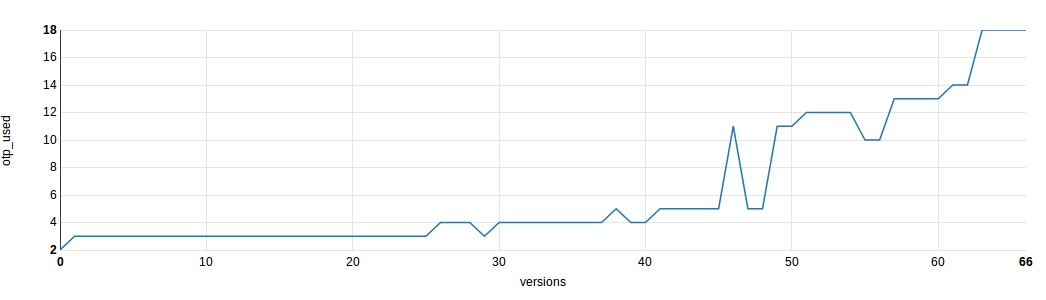
\includegraphics[width=\textwidth]{figures/otp_iron.png}
	\caption{Otp used for fe.erl file.}
	\label{fig:otp_iron}
\end{figure}

The Figure \ref{fig:mcCabe_iron} shows an overview of the evolution of the overall McCabe cyclomatic complexity. We can observe that the complexity keeps increasing.

There was a spike in 45th version, because some functions were called to an other module, however author removed changes in 46th version. There was also an insignificant drop in complexity in 28th version and a little increase in 29th version. The  complexity decreases  when  the  extracted  piece  of code occurred more than one time and the complexity of the function is more than one ~\cite{mcCabe}. 

In Figure \ref{fig:max_depth_of_cases_iron} we can see that the metric \textbf{max\_depth\_of\_cases} is 1, but before it was 0, therefore developer stopped using case inside another case for this version of the software. We can find the same trend on plot with \textbf{mcCabe} metric where it appears as decreasing of the program complexity.  

\begin{figure}[ht]
	\centering
	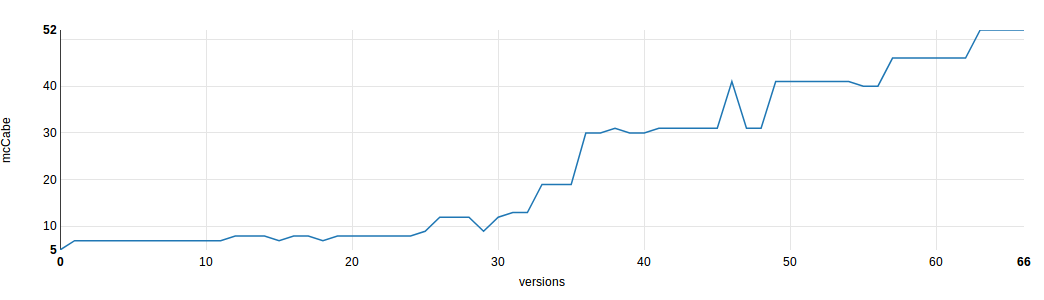
\includegraphics[width=\textwidth]{figures/mcCabe_iron.png}
	\caption{McCabe cyclomatic complexity metric for fe.erl file.}
	\label{fig:mcCabe_iron}
\end{figure}

\begin{figure}[ht]
	\centering
	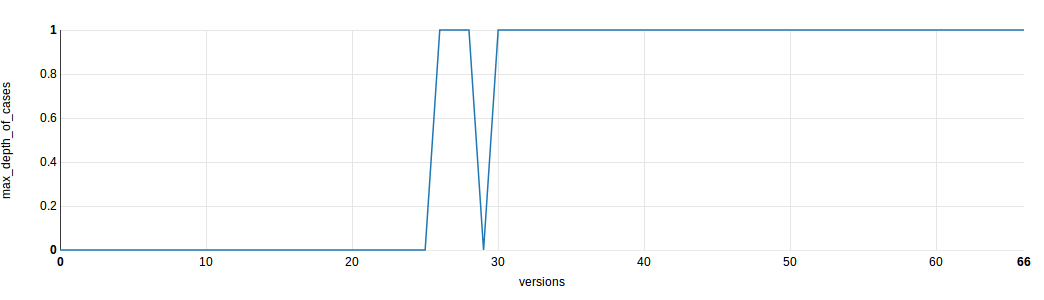
\includegraphics[width=\textwidth]{figures/max_depth_of_cases_iron.png}
	\caption{Max depth of cases for fe.erl file.}
	\label{fig:max_depth_of_cases_iron}
\end{figure}

The average length of the line was not stabilized until 35th version with gradually decreasing from 50 symbols to 38 symbols in Figure \ref{fig:average_length_of_line_iron}.

\begin{figure}[ht]
	\centering
	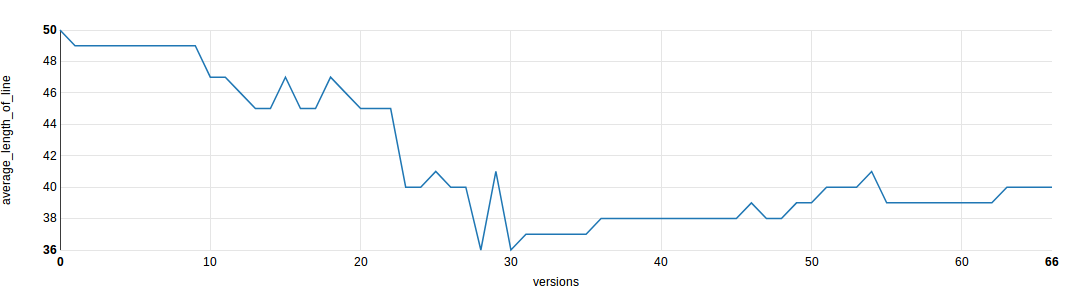
\includegraphics[width=\textwidth]{figures/average_length_of_line_iron.png}
	\caption{Average length of line for fe.erl file.}
	\label{fig:average_length_of_line_iron}
\end{figure}

As we can see in Figure \ref{fig:number_of_macros_iron} and Figure \ref{fig:number_of_records_iron} there are not defined macroses and records in the whole iron project.

\begin{figure}[ht]
	\centering
	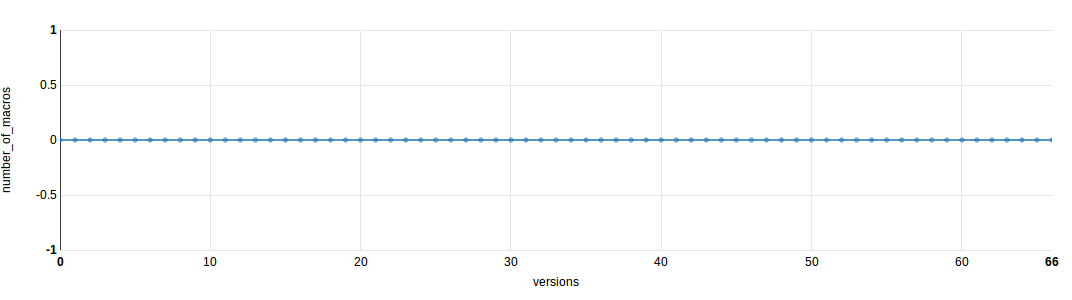
\includegraphics[width=\textwidth]{figures/number_of_macros_iron.png}
	\caption{Number of macros for fe.erl file.}
	\label{fig:number_of_macros_iron}
\end{figure}

\begin{figure}[ht]
	\centering
	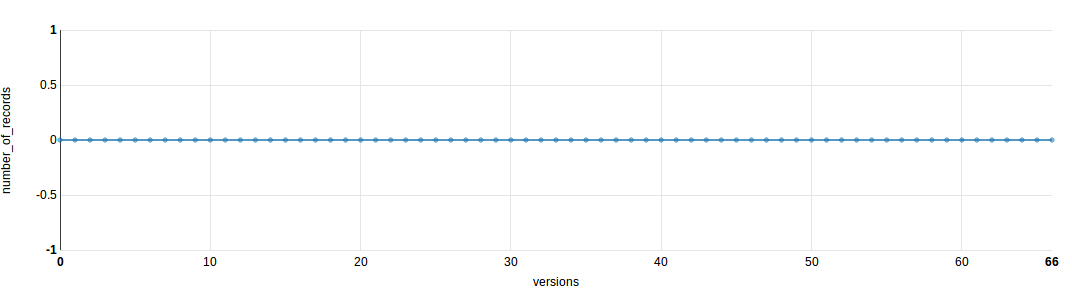
\includegraphics[width=\textwidth]{figures/number_of_records_iron.png}
	\caption{Number of records for fe.erl file.}
	\label{fig:number_of_records_iron}
\end{figure}
%%____________________________________________________________________-

\section{Erlang chat }

This project is multi-user chat written in Erlang. It has nine source code files and 45 commits. The link to the repository is \url{https://github.com/bildeyko/erlangChat}.

For this project, we analyzed the module \textbf{websocket\_handler.erl}. This module consists of 6 functions.

We can see an increasing number of lines of code in Figure \ref{fig:loc_chat} and an increasing number of characters in a program text in Figure \ref{fig:char_of_code_chat}.

\begin{figure}[ht]
	\centering
	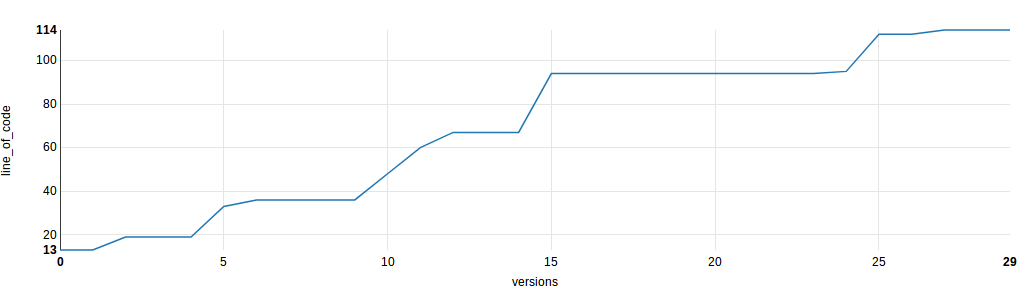
\includegraphics[width=\textwidth]{figures/loc_chat.png}
	\caption{Effective Line of code for module websocket\_handler.erl.}
	\label{fig:loc_chat}
\end{figure}

\begin{figure}[ht]
	\centering
	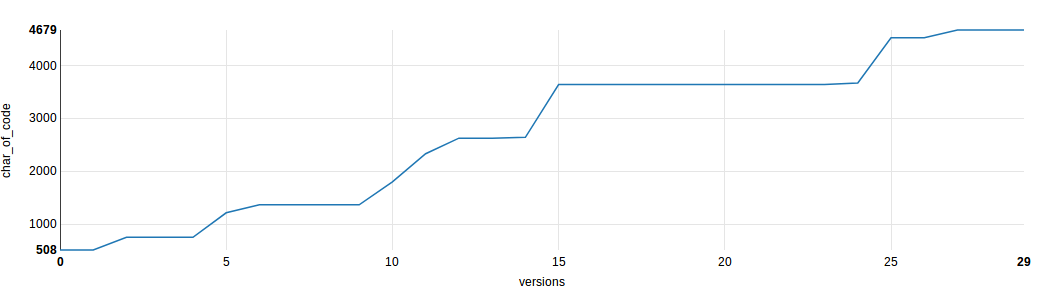
\includegraphics[width=\textwidth]{figures/char_of_code_chat.png}
	\caption{Characters of the code for module websocket\_handler.erl.}
	\label{fig:char_of_code_chat}
\end{figure}

In Figure \ref{fig:chat} we can see that the author started using message passing from the 9th version of his software.

\begin{figure}[ht]
	\centering
	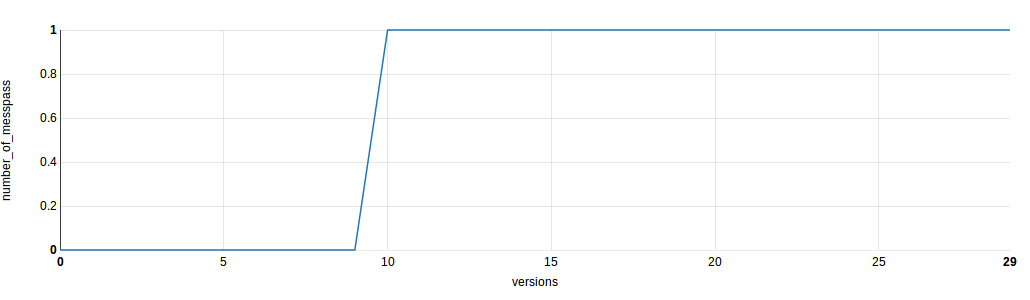
\includegraphics[width=\textwidth]{figures/chat.png}
	\caption{The number of message passing for module websocket\_handler.erl.}
	\label{fig:chat}
\end{figure}

As shown in Figure \ref{fig:chat5} there was increase in the length of the longest line of code in 9th version. 
\begin{figure}[ht]
	\centering
	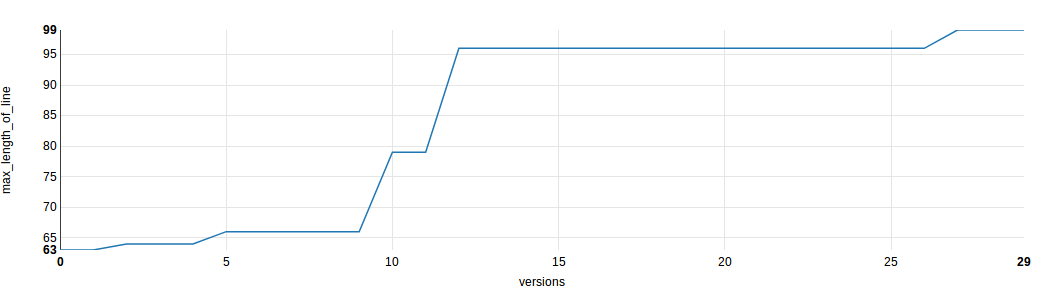
\includegraphics[width=\textwidth]{figures/chat5.png}
	\caption{Max length of line for module websocket\_handler.erl.}
	\label{fig:chat5}
\end{figure}

McCabe’s cyclomatic complexity metric measurement guarantees that developers are sensitive to the fact that programs with high McCabe numbers, for example, more than 10 are likely to be hard for understanding and accordingly have a higher probability of defects containing within the code base. The tested module has the cyclomatic complexity number which increased to 30 in the last versions as shown in Figure \ref{fig:mcCabe}.

\begin{figure}[ht]
	\centering
	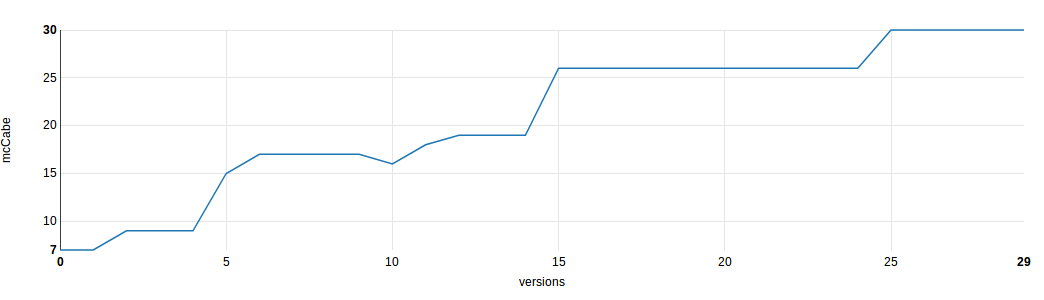
\includegraphics[width=\textwidth]{figures/mcCabe.png}
	\caption{
	McCabe cyclomatic complexity metric for module websocket\_handler.erl.}
	\label{fig:mcCabe}
\end{figure}

In Figure \ref{fig:chat2} shows that developer used otp library functions but after 9th version reconsidered to use them.

\begin{figure}[ht]
	\centering
	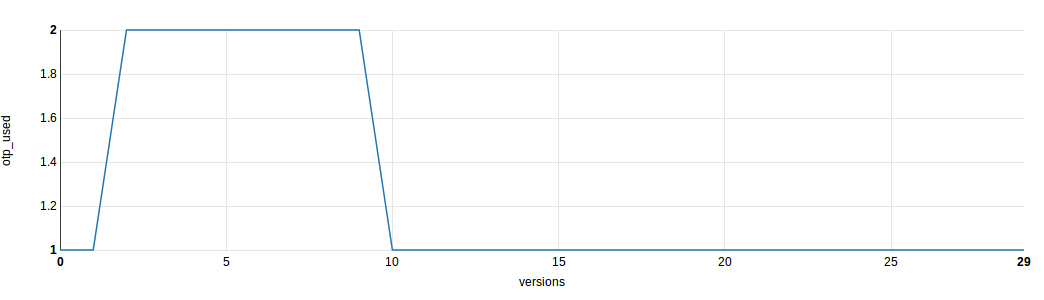
\includegraphics[width=\textwidth]{figures/chat2.png}
	\caption{Otp used for websocket\_handler.erl.}
	\label{fig:chat2}
\end{figure}

The developed framework allows measuring and visualizing metrics for a module and also for each function in the module. For example, in this module developer use message passing from the 9th version as we mentioned above. The Figure \ref{fig:chat3} shows that there was discovered function in which the author actively used message passing.

\begin{figure}[ht]
	\centering
	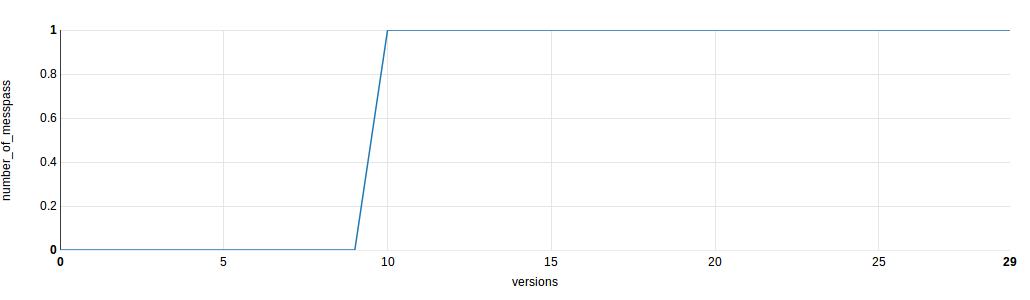
\includegraphics[width=\textwidth]{figures/chat3.png}
	\caption{Number of message passing for function websocket\_handle/3.}
	\label{fig:chat3}
\end{figure}

Visualizing of metrics helps to find which functions have been changed, added or deleted. As shown in the Figure \ref{fig:chat3} the developer slightly changed the function \textbf{terminate/3} by adding two lines of code in the 9th version.

\begin{figure}[ht]
	\centering
	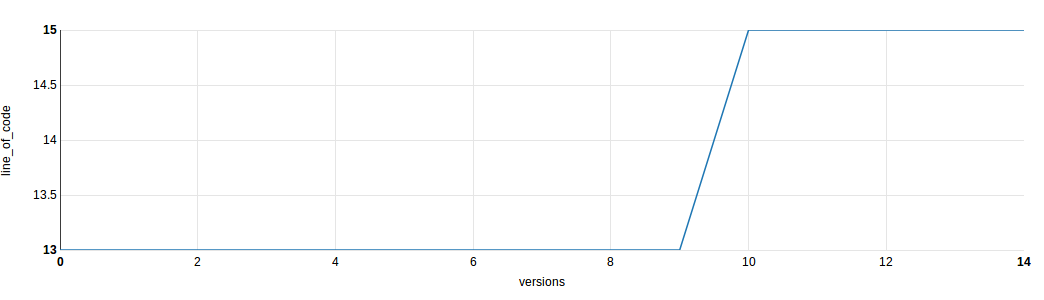
\includegraphics[width=\textwidth]{figures/chat4.png}
	\caption{
		Effective lines of code for function terminate\_/3.}
	\label{fig:chat4}
\end{figure}
 
To summarize findings we can assume that most of these changes were done in the 9th version.

%%______________________________________________________

\section{prx}

This project is an Erlang library for Unix process management and system programming tasks. Code from all project is divided into 4 modules. 

The project provides:

\begin{itemize}
	\item Reliable operating system process management by mapping Erlang processes to a hierarchy of system processes.
	\item Beam-friendly interface for system calls and other POSIX operation.
	\item Operations for processes isolation like jails and containers.
	\item An interface for separation operations with privileges for processes restriction.
\end{itemize}


The link to the repository is \url{https://github.com/msantos/prx}. This project has 201 commits. 

For this project, we tested the module \textbf{prx.erl}. 

As in previous two experiments, at the beginning, we started to measure the \textbf{LOC} metric. This metric helps us to see the changes all of the project from over time. This result is shown in Figure \ref{fig:line_of_code_prx}.

\begin{figure}[ht]
	\centering
	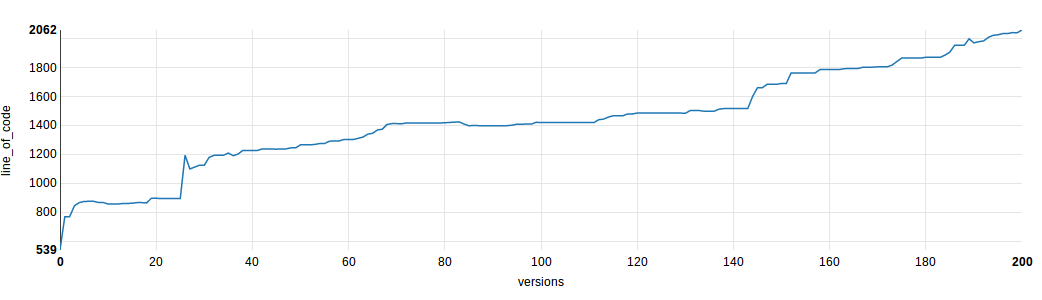
\includegraphics[width=\textwidth]{figures/line_of_code_prx.png}
	\caption{Effective Line of code for module prx.erl.}
	\label{fig:line_of_code_prx}
\end{figure}

Another important metric is \textbf{cohesion} metric. Modules with large cohesion number is preferable because high cohesion is associated with many desirable attributes of software such as robustness, reusability, reliability, and understandability. Otherwise, low cohesion is associated with undesirable attributes, for example, being difficult to reuse, maintain, test, or even understand. The Figure \ref{fig:cohesion_prx} and shows the decreasing of the calculated metric. 

\begin{figure}[ht]
	\centering
	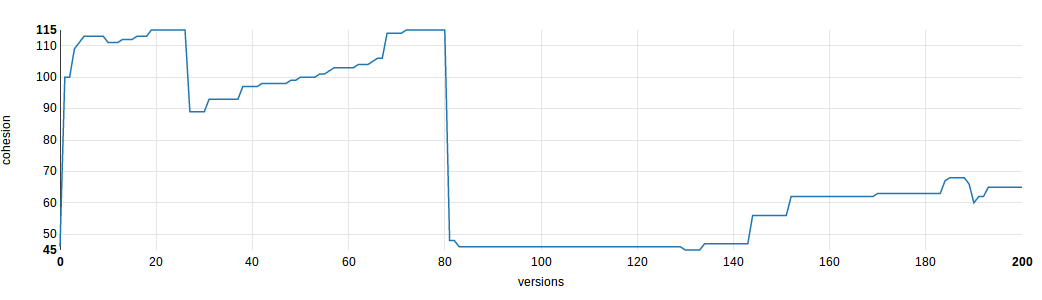
\includegraphics[width=\textwidth]{figures/cohesion_prx.png}
	\caption{The cohesion of the module prx.erl.}
	\label{fig:cohesion_prx}
\end{figure}

When developer started to use otp library in this project in 80th version, as we can see in Figure \ref{fig:otp_prx}, the McCabe cyclomatic complexity metric was rapidly increased in Figure \ref{fig:McCabe}. If complexity is increasing dramatically between versions, it is an indication of logic 
being added. 

\begin{figure}[ht]
	\centering
	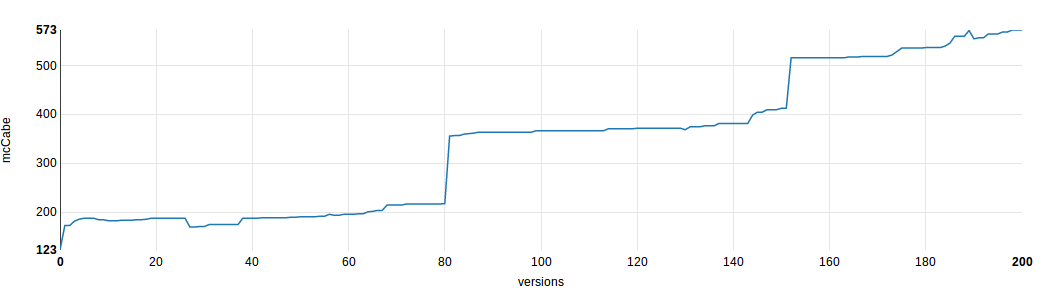
\includegraphics[width=\textwidth]{figures/mccabe.png}
	\caption{McCabe for the module prx.erl.}
	\label{fig:McCabe}
\end{figure}

When we are comparing results of cohesion and McCabe cyclomatic complexity metrics, we can conclude that low cohesion increases complexity, thereby increasing the likelihood of errors during the development process.

\begin{figure}[ht]
	\centering
	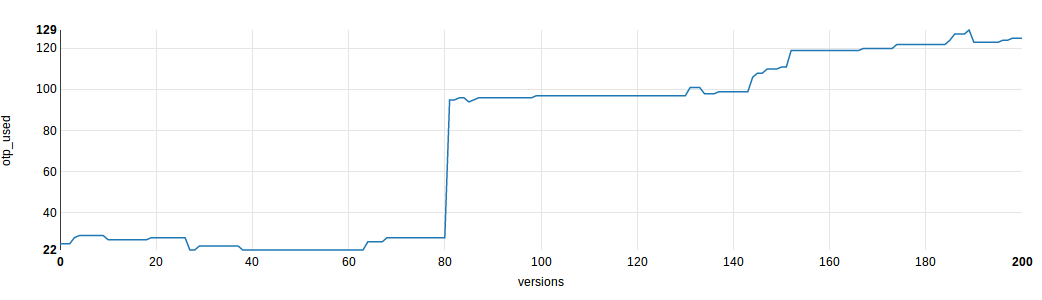
\includegraphics[width=\textwidth]{figures/otp_prx.png}
	\caption{OTP used for the module prx.erl.}
	\label{fig:otp_prx}
\end{figure}

Apart from analyzing the changes of the module we also can observe the changes of functions. The Figure \ref{fig:find/2} shows that the function \textbf{find/2} was used only in one version and later was renamed or deleted.

\begin{figure}[ht]
	\centering
	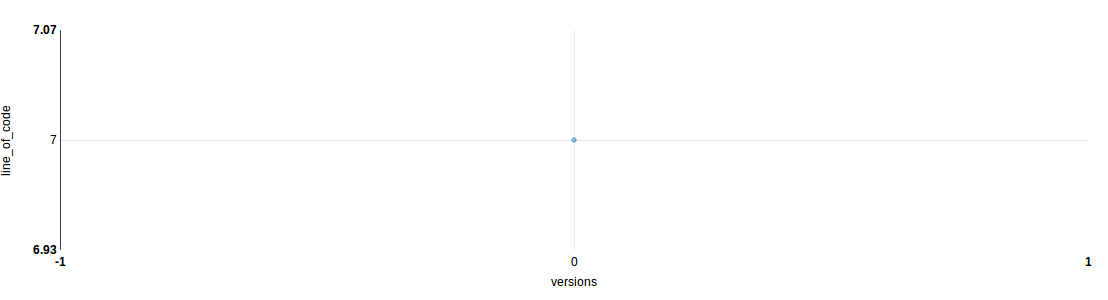
\includegraphics[width=\textwidth]{figures/find2.png}
	\caption{Effective Line of code for function find/2.}
	\label{fig:find/2}
\end{figure}

One of the features of functional programming languages is the presence of tail recursion. It is a special form of recursion where the last operation of a function is a recursive call ~\cite{tail}.
The metric \textbf{is\_tail\_recursive} returns with 1, if the given function is tail recursive; with 0, if it is recursive, but not tail recursive and -1 if it is not a recursive function. As shown in Figure \ref{fig:tail1} we can see that developer got rid of this function from 37th version until 40th version.

\begin{figure}[ht]
	\centering
	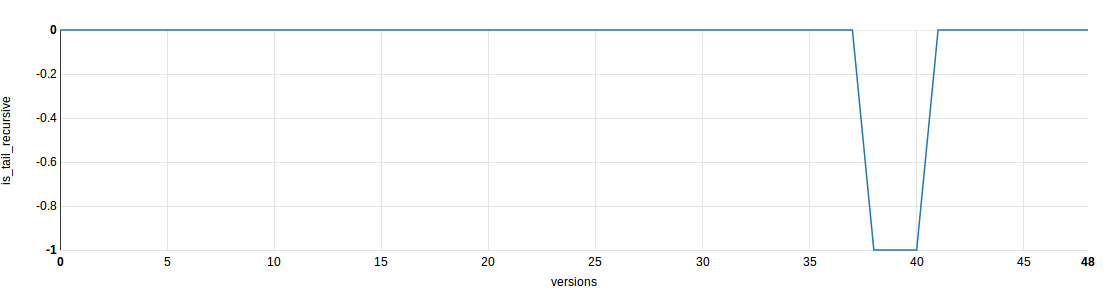
\includegraphics[width=\textwidth]{figures/filter2.png}
	\caption{Is tail recursive metric for function filter/2.}
	\label{fig:tail1}
\end{figure}

Also we can calculate how many times a function calls itself by using \textbf{branches\_of\_recursion} metric for all module. The Figure \ref{fig:br} illustrates that there were created more recursive functions after 140th version.

\begin{figure}[ht]
	\centering
	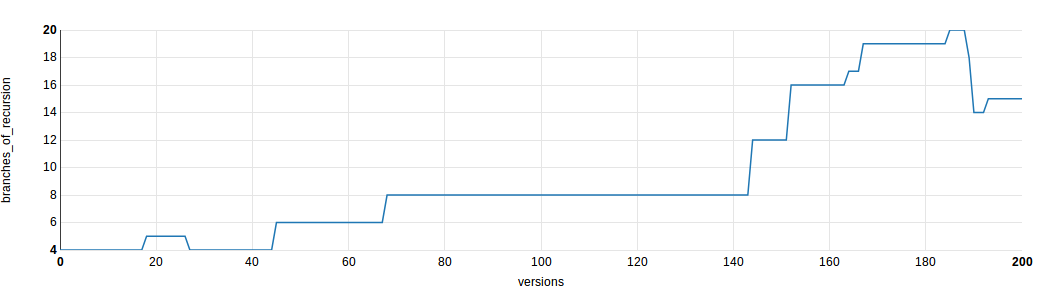
\includegraphics[width=\textwidth]{figures/br.png}
	\caption{Branches of recursion for module prx.erl.} 
	\label{fig:br}
\end{figure}

In RefactorErl there is a \textbf{function\_sum} metric which can be calculated using these metrics together: \textbf{line\_of\_code}, \textbf{char\_of\_code}, \textbf{number\_of\_funclauses}, \textbf{branches\_of\_recursion},
\textbf{mcCabe}, \textbf{calls\_for\_function}, \textbf{calls\_from\_function}, \textbf{fun\_return\_points}, \textbf{number\_of\_messpass}. Metrics \textbf{calls\_for\_function} and \textbf{calls\_from\_function} available only for functions. We can notice the dependency of \textbf{function\_sum} (Figure \ref{fig:function_sum_task4}) on two metrics changes: number of lines of code (Figure \ref{fig:task4}) and calls from the function (Figure \ref{fig:calls_from_function_task4}).

\begin{figure}[ht]
	\centering
	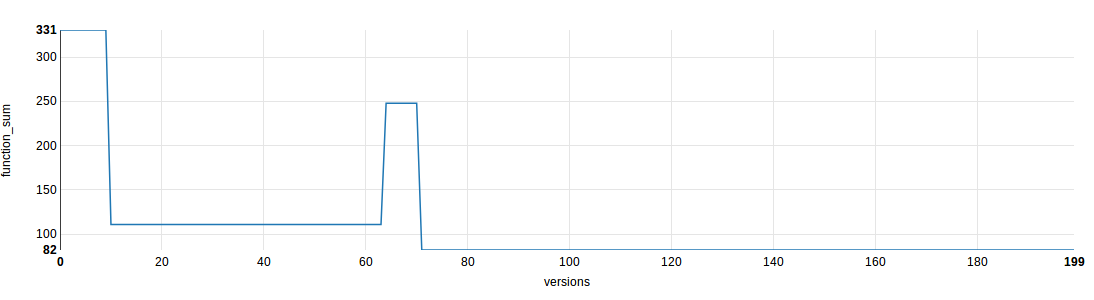
\includegraphics[width=\textwidth]{figures/function_sum_task4.png}
	\caption{Function sum function task/4.} 
	\label{fig:function_sum_task4}
\end{figure}

\begin{figure}[ht]
	\centering
	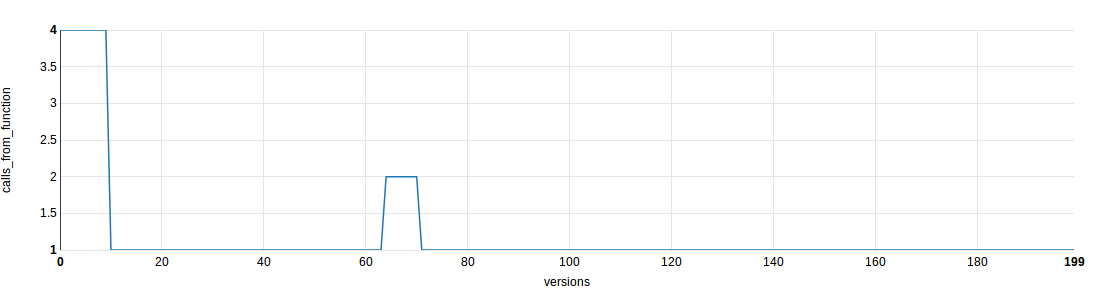
\includegraphics[width=\textwidth]{figures/calls_from_function_task4.png}
	\caption{Calls from the function for function task/4.} 
	\label{fig:calls_from_function_task4}
\end{figure}

\begin{figure}[ht]
	\centering
	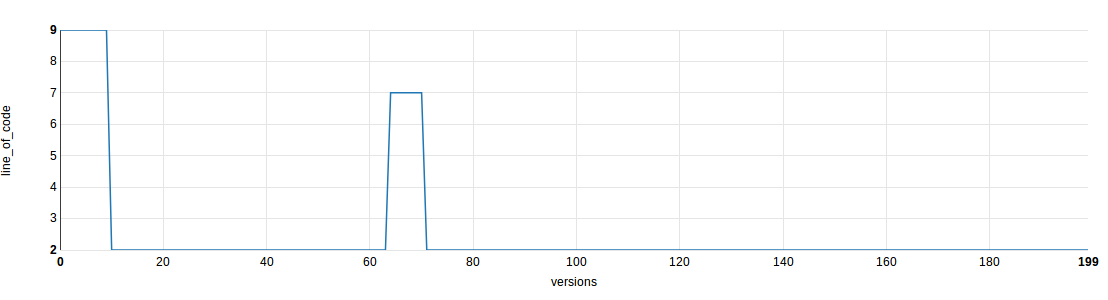
\includegraphics[width=\textwidth]{figures/task4.png}
	\caption{Effective Line of code for function task/4.} 
	\label{fig:task4}
\end{figure}

\chapter{Related work}
Nowadays, the need for the visualization of software quality metrics has been rapidly increased. Software metrics help developers and companies to check and analyze information about the performance, quality of code and cost of software data. it helps to find out and fix errors in the early stages of development.

In this chapter will be described some tools for visualization of software quality metrics and tool for code analysis.

\section{Open Source tool "METRIX"}

This tool can compute different software quality metrics. METRIX is able to evaluate software written in C and ADA languages and many metrics can be considered for software evaluation (the different metrics will be described in detail in the next section~\cite{metrix}. 

The user can use different types of diagrams for metrics visualization: histograms, scatter plots and line charts. 
This tool allows to use two not common classes of diagrams: 

\begin{itemize}
	\item The first is Kiviat diagrams, also known as the radar plots.
	\item The second is the city map diagram.
\end{itemize}

One specific feature of METRIX is to use those two types of visualization for constructing signature and cartography of source codes~\cite{metrix}.
 
\textbf{Kiviat diagrams}
The Kiviat diagram uses polar coordinates for visualization. The value which user wants to represent associated with the distance between the point and the origin. The angle between two points does not change because it is constant. This constant is calculated to uniformly distribute the different points. Linked together metric points make a plain polygon, which forms the data specifics of represented values. This type of diagram can be used only for visualization of more than three values of calculated metric. All values must be strictly positive. The user can merge data in one diagram. Also, this tool allows drawing the diagram for one or several metrics together. 

In figure\ref{fig:metrix} shows an example of two Kiviat diagrams. These diagrams represent different metric values for two functions. 

\begin{figure}[h]
	\centering
	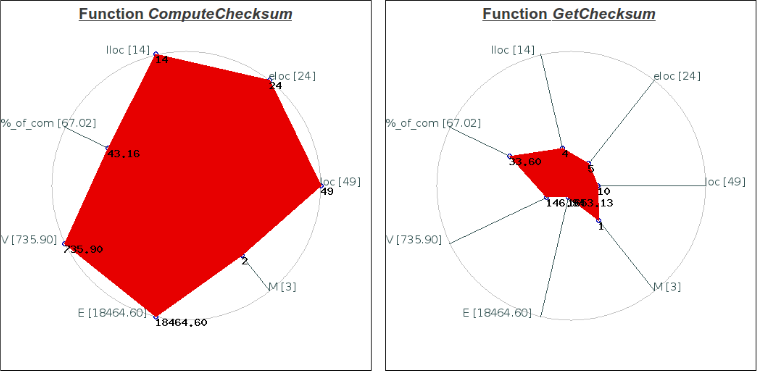
\includegraphics[height=70mm]{figures/metrix.png}
	\caption{An example of Kiviat diagrams.}
	\label{fig:metrix}
\end{figure}

\textbf{City map diagrams}
Usually this type of diagrams used for representing cities with buildings in three dimensions. City map diagrams also suit for visualization of software metrics of the project with a large number of source files, functions and variables. Source code metrics are represented by rectangles by using the treemap diagram. Some authors used variants of this class of visualization diagrams to represent  values with esthetic considerations. City map diagrams are indeed multi-parameters diagrams: each “building” is associated with an n-tuple of numeric values~\cite{metrix}.  

This tool also has a graphical user interface with a single Window containing three tabs: “Calc”, “Csv” and “Plots”.

In the first "Calc" tab user chose source files for evaluation and also chose metrics which neede to be measured.It allows to users to use  hand-start scripts with a prompt. The open source aspect of the tool allows users to repeat the measuring scripts manually or to integrate them into other software.

In the second “Csv” tab user can find a list of numeric values and chose which values will be used for function or for the file. There is an option for exporting calculated values to a spreadsheet application for drawing graphs, like scatter plots, line plots, etc.

In the third “Plots” tab the user can build the city map diagrams for the source code. The user can change the settings of the tool like the modification of placement of the buildings in the city map or make the data colored, etc.

This tool supports making a report in the form of a LaTeX file where each function and each file make a section of this report. User can use PDF file for analisis. This report includes all the values measured on the project. Each file produces three views of the associated city map diagram, as well as different Kiviat diagrams for the different metrics measured on the functions of the file~\cite{metrix}. 

\section{Sextant}

Sextant is a Java source-code analysis tool under development at the University of Nebraska at Omaha (UNO)~\cite{sextant}. This software is a complex extension of the TL system (a general-purpose program transformation system) created particularly for the Java programming language domain.

The main design goal of Sextant is providing a tool facilitating specification and visualization of custom analysis rules, which can be domain-specific or moreover application specific analysis rules.

Analysis rules of Sextant are based on information fetched from different software models. There are two main models of central importance. The first model is a syntactic model. It is the source code parse tree. Parse trees conform to compilation units which represented by Java files and are generated with use of GLR parser technology provided by the TL system. Parse trees are well-fitted for analyzing and manipulating through standard primitives provided by program transformation systems, for example, by matching and generic traversal.

The second model is a compound attributed graph (CAG). It is a semantic model which captures subtype, structural, and reference dependencies among the constructors, methods, fields, packages and types. The CAG also links an attribute list with every node and edge.

CAG information is accessible to Sextant’s transformation-based analysis rules via two mechanisms. The first mechanism is a positional system which organizes a relation between contexts within the CAG and corresponding parse (sub)trees. This relation makes possible correctly resolving references to constructors, methods, types, fields, and local variables, during the process of generic traversals which are the key enabling mechanism in program transformation systems.

The second mechanism is a library of semantic queries. These queries can be accessed even in the middle of transformation course. Functionality which provided by this library contains things like:
\begin{itemize}
	\item Reference resolving.
	\item Reference type determining.
	\item Determining declaration shadowing or overriding.
	\item Determining whether one type is a subtype of another.
\end{itemize}
 
Sextant stores table and set types for information collecting with relation to analysis rules. These constructs can be used for storing information related to a custom metrics wide variety.

Sextant is open-ended with respect to the definition of metrics – any source-code analysis rule can be interpreted as a metric, be they PMD-style rules focusing on violations of coding conventions or rules such as those specified by FindBugs that are more semantic in nature\cite{sextant}.

Sextant can do software models generation. These models can be visualized using other tools such as GraphViz, Cytoscape and TreeMap. Sextant can produce the CAG of the code base in a JavaScript object notation format (JSON). This JSON file can be loaded into Cytoscape, an open source platform which provides extensive and sophisticated capabilities for large complex networks visualization, for example, graph structures. The same way, metrics derived from sets and tables can be produced in CSV format and viewed with use of TreeMap. Parse trees can be output as dot-files and later viewed with use of GraphViz.

The view in Figure\ref{fig:1} shows an example of represents a coloring of dependencies on the unsupported features. Nodes colored orange have indirect dependencies on unsupported features while purple nodes have direct dependencies on unsupported features.

\begin{figure}[h]
	\centering
	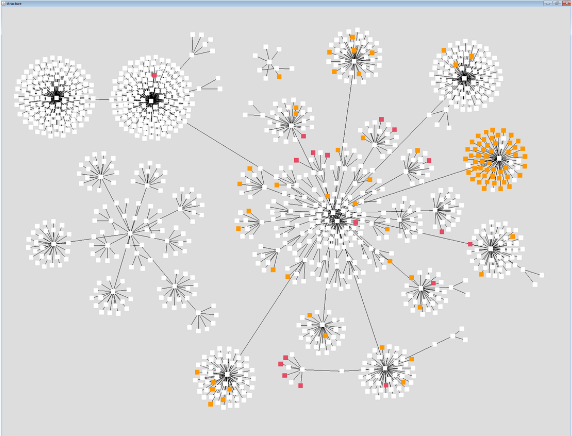
\includegraphics[height=70mm]{figures/1.png}
	\caption{An example of using Sextant tool.}
	\label{fig:1}
\end{figure}

\section{NDepend}

NDepend is a static analysis tool for .NET managed code. The tool supports a big number of code metrics, allowing to visualize dependencies using directed graphs and dependency matrix.  

NDepend computes a lot of size-related metrics: number of lines of code, number of assemblies, number of types, number of methods, etc. For measuring complexity, NDepend uses Cyclomatic Complexity. This metric measures the complexity of a type or a method by calculating the number of branching points in the code.
NDepend has two metrics for cohesion. Relational Cohesion is an assembly level metric that measures the average number of internal relationships per type. Lack of Cohesion Of Methods (LCOM) measures the cohesiveness of a type. A type is maximally cohesive if all methods use all instance fields.

NDepend uses a visualization tool called a Treemap.
NDepend comes with a dashboard to quickly visualize all application metrics s shown in Figure\ref{fig:dash}. The dashboard is available both in the Visual Studio extension. For each metric, the dashboard shows the diff since baseline. It also shows if the metric value gets better (in green) or wort (in red). 

\begin{figure}[h]
	\centering
	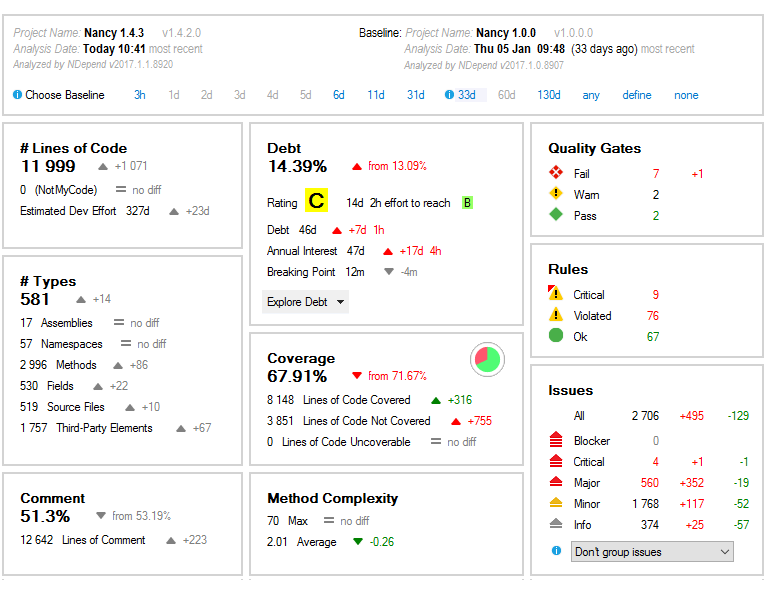
\includegraphics[height=70mm]{figures/dash.png}
	\caption{An example of using the dashboard.}
	\label{fig:dash}
\end{figure}

The Figure\ref{fig:tree} shows metric visualization using the colored treemap.

\begin{figure}[h]
	\centering
	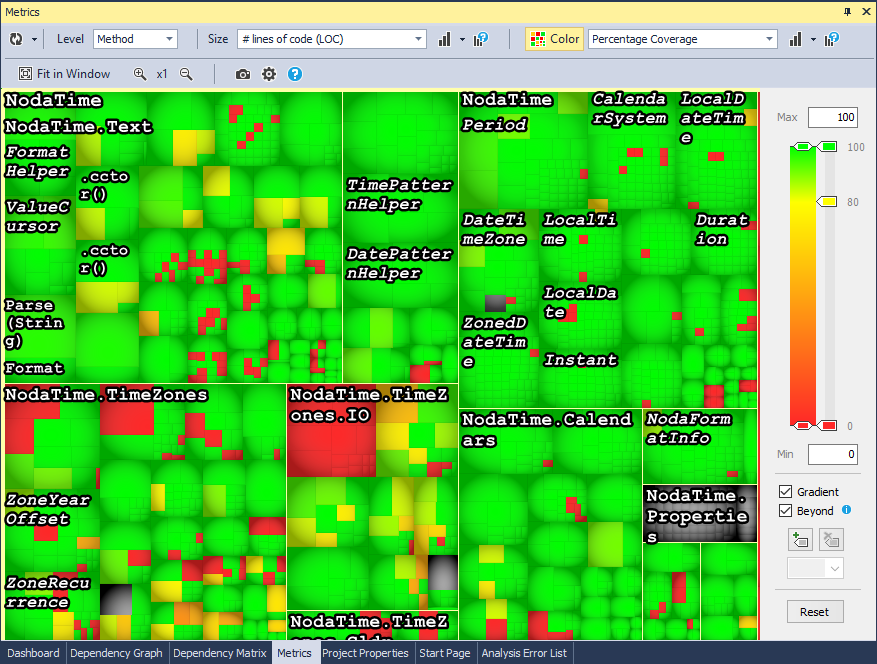
\includegraphics[height=70mm]{figures/tree.png}
	\caption{An example of using the colored treemap.}
	\label{fig:tree}
\end{figure}

The tree structure used in NDepend treemap is the usual code hierarchy: 

\begin{itemize}
	\item .NET assemblies contain namespaces.
	\item Namespaces contain types.
	\item Types contain methods and fields.
\end{itemize}

\section{PVS-Studio}

PVS-Studio is a tool for detecting bugs and security weaknesses in the source code of programs, written in C, C++, and C\#. It works in Windows, Linux, and macOS environment~\cite{pvs}. The user can use online reference manual concerning all the diagnostics methods available in the program and  on the website.

This tool executes static code analysis. The generated report helps developers in debugging. PVS-Studio has large number of methods for checking. These methods help to find typing and copy-paste mistakes. The main value of static analysis is in its regular use so that errors are identified and fixed at the earliest stages~\cite{pvs}. 				

PVS-Studio can work on a Linux environment on Windows. It can be run from the command or can be integrated into Visual Studio development environment. The results of the analysis are presented in the HTML document which allows full navigation through the source code. The Figure \ref{fig:pvs} shows an example of HTML-report.

\begin{figure}[h]
	\centering
	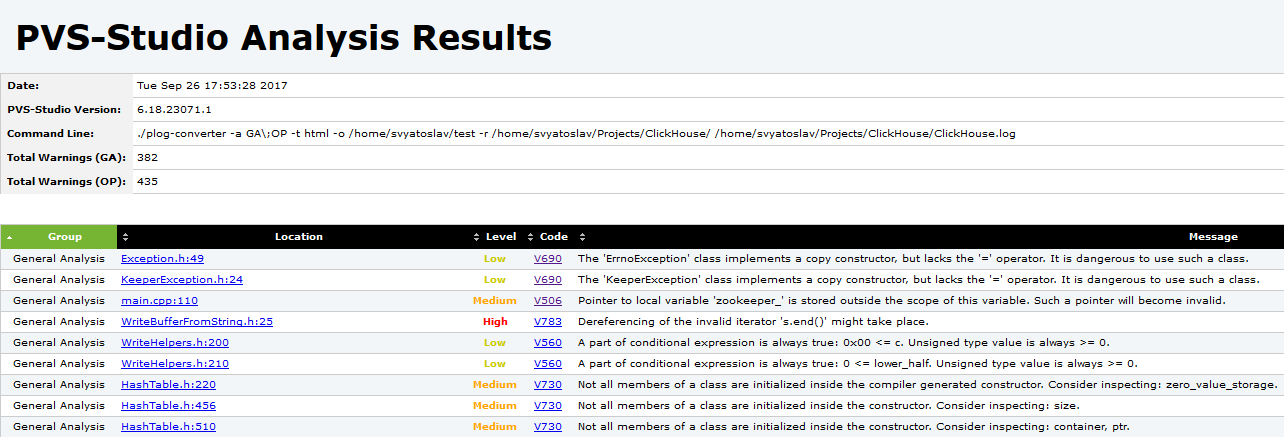
\includegraphics[height=53mm]{figures/pvs.png}
	\caption{Main page of an HTML-report.}
	\label{fig:pvs}
\end{figure}

It is possible to not include files from the analysis by name, folder or mask; to run the analysis on the files modified during the last N days~\cite{pvs}. PVS-Studio has an integration with open source platform SonarQube. This platform was designed for uninterrupted analysis and evaluation of the quality of code.

\chapter{Conclusion}
The main goal of this thesis, as stated at the beginning of this work, is to analyze the quality of programs written in the Erlang programing language by using RefactorErl tool. To accomplish that goal, it became necessary to provide a general overview of Erlang, RefactorErl static analysis tool and developed metrics. In this thesis, the software quality, software metrics and some of the tools for measuring software quality metrics have been studied and analyzed.

Erlang is a functional language designed for highly parallel, scalable applications requiring high uptime ~\cite{refactorerlimp}. RefactorErl ~\cite{refactorerl} is a static source code analysis and transformation tool for Erlang providing several software metrics. The tool is developed by the Department of Programming Languages and Compilers at the Faculty of Informatics, Eötvös Loránd University, Budapest, Hungary. Among the features of RefactorErl is included a metric query language which can support Erlang developers in everyday tasks such as program comprehension, debugging, finding relationships among program parts, etc.

In this thesis, we presented a developed framework which analyzes git repositories with Erlang code files. The new component is built on RefactorErl static analysis tool and actively uses its feature of calculating different metrics of Erlang modules and functions. This framework allows drawing plots which show change of metrics with software evolving from version to version. The plots can be saved for future usage as a pictures in PNG format. 

The main focus of the component is to help Erlang developers with analyzing their projects using plots. Also, it was important to test the developed component on some projects and after that to analyze the measurements. For this purpose have been chosen three different projects from git. The experimental results allow finding changes (increasing the line of code number, char of code number, using otp library and etc.) in code. Visualisation helps with finding patterns and improving of the code quality.

It is safe to say that the main goals of this thesis were successfully achieved. The usage of software metrics is within an organization and its usage is expected to have a beneficial effect on software organizations by making software quality more visible.

%%%%%%%%%%%%%%%%%%%%%%%%%%%%%%
%% Bibliography starts here %%

\addcontentsline{toc}{chapter}{Bibliography}

%% There's more than one way to keep track of your citations.

%% For simply listing the citations by text you can use the thebibliography 
%% environment. See biblio.tex for an example. Comment out the following line
%% to use this style.
  
% %% You only need to keep one of biblio.bib and biblio.tex, depending which 
%% citation managament style you want to use.

\begin{thebibliography}{10}

\bibitem{ecore}
\newblock Az EMF Ecore meta-metamodell sematikus ábrája.
\newblock \emph{Eclipse Foundation. Xtext Documentation}
\newblock \\ https://eclipse.org/Xtext/documentation/308\_emf\_integration.html
\newblock \\ 2016.04.27

\bibitem{omguml}
\newblock \emph{Object Management Group. OMG Unified Modeling Language Superstructure}
\newblock \\ www.omg.org/spec/UML/
\newblock \\ 2015.11.30.

\bibitem{refactorerl1}
\newblock \emph{Melinda Tóth \& István Bozó:
\newblock Static Analysis of Complex Software Systems Implemented in Erlang},
\newblock \\ Central European Functional Programming Summer School Fourth Summer 
School, CEFP 2011, Revisited Selected Lectures, Lecture Notes in Computer
Science (LNCS), Vol. 7241, pages 451-514, Springer-Verlag, ISSN: 0302-9743,
\newblock 2012.

\bibitem{refactorerl2}
\newblock \emph{István Bozó, Dániel Horpácsi, Zoltán Horváth, Róbert Kitlei, Judit Kőszegi, Máté Tejfel, Melinda Tóth:
\newblock RefactorErl - Source Code Analysis and Refactoring in Erlang},
\newblock \\ Proceedings of the 12th Symposium on Programming Languages and Software
Tools, ISBN 978-9949-23-178-2, pages 138-148,
\newblock \\ Tallin, Estonia,
\newblock \\ 2011.10.

\bibitem{erlangdocs}
\emph{Erlang Programming Language},
\newblock \\ http://www.erlang.org/
\newblock \\ 2015.11.30

\end{thebibliography}



%% Another way is to use bibtex. The following command will process and 
%% include the citations listed in biblio.bib. The advantage of bibtex is that
%% you can simply copy-paste citations if the authors provided a bib-citation. 
%% For examples of such bib-citations, click the small "bib" link beside the 
%% articles at  https://plc.inf.elte.hu/erlang/refactorerl-academic-results.html

\bibliography{biblio.bib}{}
\bibliographystyle{unsrt}

%%%%%%%%%%%%%%%%%%%%%%%%%%%%
%% Appendices starts here %%

\addtocontents{toc}{\setcounter{tocdepth}{0}}
\end{document}
